\documentclass{article}
\usepackage[utf8]{inputenc}
\usepackage{appendix}
\usepackage{url}
\usepackage{amssymb}    % for \checkmark
\usepackage{booktabs}  
\usepackage[most]{tcolorbox}


\title{Scenario Generation for Interactive Urban Environments}
\author{Paritosh Sharma, Hui-Yin Wu}
\date{September 2025}

\usepackage{graphicx}
\usepackage{subcaption}
\usepackage{hyperref}
\usepackage{pgfplots}
\usepackage{tikz}
\usepackage{amsmath}
\usepackage{multirow}
\usepackage{array}
\usepackage{enumitem}
\usepackage{lscape}
\usepackage{geometry} 
\usepackage{adjustbox}

\usetikzlibrary{shadows,arrows.meta,positioning,fit}

\tikzset{
  module/.style={rectangle, rounded corners=6pt, draw=orange!80!black, very thick, fill=black!90, 
                 text=white, align=left, font=\bfseries, minimum width=3.5cm, minimum height=2cm},
  subtext/.style={font=\scriptsize\color{white}, align=left},
  arrow/.style={-{Latex[length=3mm]}, thick, orange!80!black},
}

\tcbuselibrary{listings, breakable}

% Define a style for examples
\tcbset{
  examplebox/.style={
    colback=blue!3!white,
    colframe=blue!60!black,
    coltitle=black,
    fonttitle=\bfseries,
    sharp corners,
    boxrule=0.6pt,
    breakable,
    enhanced,
    left=5pt, right=5pt, top=5pt, bottom=5pt
  }
}

\begin{document}

\maketitle

\section*{Project members}

\begin{itemize}
    \item Scientific team: Paritosh Sharma, Hui-Yin Wu
\end{itemize}

\section{Context and objectives}

The document highlights the work plan for the the WP4 of the ANR Creative 3D~\footnote{\url{https://project.inria.fr/creattive3d/}} project. The expected outcome of this project is to create a generative model that is capable of creating personalized training scenarios in urban environments.

\section{Introduction}

Virtual Reality (VR) and Augmented Reality (AR) technologies have advanced significantly in recent years, enabling the creation of immersive and interactive environments for various applications. These can be further used to provide personalized training and rehabilitation scenarios. In the context of low vision rehabilitation, these models can be particularly useful to study pedestrian behaviours under normal and simulated vision. However, most simulated environments suffer from perceptual gaps between the designer, the user, and the system. The existing GUsT-3D framework~\cite{wu2022designing}, developed during the Creative3D project, provides a foundation to address this. However, the current framework is still limited by its reliance on a fixed set of urban environments and interactions innhibiting its ability to scale.

In parallel, recent works on 3D generative models for urban scenario generation has shown promising results in generating diverse and realistic urban environments. Additionally, these models have been able to capture the diverse nature and the complexities of an urban setting, including the interactions between pedestrians, vehicles, and the environment. Driven by these extraordinary capabilities, exploring the potential of generative models will enable us to create more diverse and realistic urban scenarios.

\section{Related Work}

In this section, we first start by reviewing prior work on pedestrian-in-the-loop simulations. Then, we review recent works on generative models for urban scenario generation as well as diffusion-based 4D generation. Finally, we discuss common validation methods used to evaluate the performance of these models.

\subsection{Pedestrian-in-the-Loop}

VR Simulations have been widely used to study pedestrian behavior and interactions in urban scenarios~\cite{wu2018using,tran2021review,mukoya2024jaywalkervr,schneider2020virtually}. This human-in-the-loop approach (also referred as pedestrian-in-the-loop\cite{hartmann2017pedestrian}) allows researchers to collect data on how pedestrians interact with their environment, including their decision-making processes, movement patterns, and responses to various stimuli. These simulations can be used to study a wide range of scenarios, from simple road crossings to complex urban environments with multiple interacting agents. More recently, JaywalkerVR~\cite{mukoya2024jaywalkervr}, a VR human-in-the-loop simulator, used CARLA~\cite{dosovitskiy2017carla} to create four different scenarios: jaywalking, parked cars, four-way stops, and parking lot entrances. Despite the obvious advantages, developing such simulators is still challenging because of the perceptual gaps between the designer, the user and the system as identified by Dourish~\cite{dourish2001action}.

The GUsT-3D framework~\cite{wu2022designing} addresses this by first defining the scene using a scenegraph, which captures the relationships between different elements in the scenario (ontology) and then defining the task to be carried out during the course of the scenario using a GUTasks (intersubjectivity). Lastly, it uses a query component for logging and post-scenario analysis of the experience (intentionality). This framework was also applied by creating a dataset of 6 road-crossing scenarios to study pedestrian behavior under normal and low vision~\cite{wu2023exploring}. Even though GusT-3D framework addresses the perceptual gaps which were identified by Dourish, it still relies on a fixed set of scenarios and interactions.

\subsection{Generative Models for Urban Scenario Generation}

\subsubsection{Image-based Generation}

Diffusion models have shown impressive results in generating high-quality images from textual descriptions. Models like DALL-E 2~\cite{ramesh2022hierarchical}, Imagen~\cite{saharia2022photorealistic}, and Stable Diffusion~\cite{rombach2022high} have demonstrated the ability to create diverse and realistic images based on text prompts. Recent works such as GameNGen~\cite{valevski2024diffusion}, Genie~\cite{bruce2024genie}, and DIAMOND~\cite{alonso2024diffusion} have shown the potential of diffusion models to generate game environments in real-time. However, these models suffer from latency issues since they are not truly 3D and generate image-by-image.


\subsubsection{Prompts}

Prompts are textual cues provided to the generative model to guide the scenario creation process. Since the popularity of LLMs like GPT-3, prompts have become a common way to interact with generative models. They can be used to specify the desired characteristics of the scenario, such as the type of environment, objects, and their relationships. Table \ref{tab:prompt_based_models} lists some of the recent prompt-based models for scenario generation.

\begin{table}[h]
\centering
\resizebox{\textwidth}{!}{
    \begin{tabular}{|c|c|c|}
    \hline
    \textbf{Model} & \textbf{Technique} & \textbf{Output} \\ \hline
    ScenicNL~\cite{elmaaroufi2024scenicnl} & Converts LLM Prompts to Scenic Constraints & Scenic Scenario \\ \hline
    ChatScene~\cite{zhang2024chatscene} & Conversational Agent for Scenario Definition using Scenic & Scenic Scenario \\ \hline
    LayoutGPT~\cite{feng2023layoutgpt} & Prompts converted to CSS-like Layout Formatting by LLMs & Layout Representation \\ \hline
    ChatDyn~\cite{wei2024chatdyn} & LLM-based planning and low-level trajectory generation for Pedestrian and Vehicle & 3D Scenario \\ \hline
    Work by Feng et al.~\cite{feng2025text} & JSON to describe layout and 3D models & 3D Scene \\ \hline
    TTSG~\cite{ruan2024traffic} & LLM-based planning and retrieval & 3D Scenario \\ \hline
    3D-SceneDreamer~\cite{zhang20243d} & Prompt to point-of-view image followed by image to 3D & 3D Scene \\ \hline
    GraphCanvas3D~\cite{liu2024graph} & Uses LLM to create a scenegraph and then a 3D scene & 3D Scene \\ \hline
    Scenethesis~\cite{ling2025scenethesis} & Uses LLM to create a scenegraph and then a 3D scene & 3D Scene \\ \hline
    SceneX~\cite{zhou2024scenex} & LLM to plan PCG (Procedural Controllable Generation) & 3D Scene \\ \hline
    Surreal Drivers~\cite{jin2024surrealdriver} & Chain-of-thought prompts & 3D Scene \\ \hline
    Text2nerf~\cite{zhang2024text2nerf} & Text prompts & 3D Scene \\ \hline
    X-Scene~\cite{yang2025x} & Text prompts & 3D Scene \\ \hline
    \end{tabular}
}
\caption{Prompt-based Models for Urban Scenario Generation}
\label{tab:prompt_based_models}
\end{table}

\subsubsection{Layout-guided Generation}

Layouts are structured representations of scenarios that capture the spatial relationships between different elements, such as buildings, roads, and pedestrians. These may include bird's-eye views, top-down maps, or other forms of spatial representations that provide a high-level overview of the scenario. Table~\ref{tab:layout_based_models} lists some of the recent layout-based models for scenario generation.

\begin{table}[ht]
\centering
    \begin{tabular}{|c|c|c|}
    \hline
    \textbf{Model} & \textbf{Technique} & \textbf{Output} \\ \hline
    CC3D~\cite{bahmani2023cc3d} & 2D Layout-based 3D Scene Generation & 3D Scene \\ \hline
    CityDreamer4D~\cite{xie2025citydreamer4d} & Uses a Layout Generator and a traffic scenario generator & 3D Scenario \\ \hline
    Infinicube~\cite{lu2024infinicube} & Text prompts, HD Maps and Bounding Boxes & 3D Scenario \\ \hline
    Work by Zhang et al.~\cite{urbandiff} & BEV map & 3D Scene \\ \hline
    UniScene~\cite{li2025uniscene} & BEV map & Multi-view video \\ \hline
    Savkin et al.~\cite{savkin2021unsupervised} & Scenegraph & Scenario Image \\ \hline
    \end{tabular}
\caption{Layout-based Models for Urban Scenario Generation}
\label{tab:layout_based_models}
\end{table}

Additionally, some works have also combined multimodal inputs with different types of data, prompts, layouts and other structured representations, to provide a richer context for scenario generation. Table~\ref{tab:multimodal_models} lists some of the recent multimodal models for scenario generation.

\begin{table}[ht]
\centering
\resizebox{\textwidth}{!}{
    \begin{tabular}{|c|c|c|}
    \hline
    \textbf{Model} & \textbf{Input Type} & \textbf{Output} \\ \hline
    CityX~\cite{zhang2024cityx} & Prompt, OSM file or Semantic Map & 3D Scenario \\ \hline
    CityCraft~\cite{deng2024citycraft} & Layout data and text prompts & 3D Scene \\ \hline
    Work by Liu et al.~\cite{liu2025controllable} & Scenegraph assisted using text prompts & 3D Scene \\ \hline
    GAUDI~\cite{bautista2022gaudi} & Conditioning using prompts or point-of-view images & 3D Scene \\ \hline
    MagicDrive3D~\cite{gao2024magicdrive3d} & Text prompts, Bird Eye View (BEV) map and 3D Bounding Boxes & Reconstructed 3D video \\ \hline
    Scene123~\cite{yang2024scene123} & Text prompt, point-of-view image or Text Description & 3D Scene \\ \hline
    StreetScapes~\cite{deng2024streetscapes} & BEV and height map with support for prompts & Video \\ \hline
    Urban Architect~\cite{lu2024urban} & 3D Layout and Text Prompts & 3D Scene \\ \hline
    Urban World~\cite{shang2024urbanworld} & Layout (generation) and prompts (refinement) & 3D Scenario \\ \hline
    Wonderplay~\cite{li2025wonderplay} & point-of-view image and action (physics) & 3D Video \\ \hline
    \end{tabular}}
\caption{Multimodal Models for Urban Scenario Generation}
\label{tab:multimodal_models}
\end{table}

\subsection{Validation}

Table \ref{tab:validation} lists common qualitative and quantitative validation methods used to evaluate the performance of generative models for urban road-crossing scenarios. These methods assess the quality, realism, and diversity of generated scenarios.

\begin{table}[ht]
\centering
\caption{Qualitative and Quantitative Evaluation Methods for Road-Crossing Scenarios}
\resizebox{\textwidth}{!}{
\begin{tabular}{|p{2.5cm}|p{3.5cm}|p{6.2cm}|p{4.5cm}|}
\hline
\textbf{Method Type} & \textbf{Evaluation Approach} & \textbf{Description} & \textbf{Use Case} \\
\hline

\multirow{5}{*}{Qualitative}
& Human Review & Human experts assess realism, scenario diversity, and layout plausibility. & Validates human-perceived quality and applicability of the scene. \\
\cline{2-4}
& Scenario Visualization & 3D visual inspection or rendered videos showing pedestrian, vehicle, and environment interactions. & Helps detect unrealistic or unnatural behavior/configurations. \\
\cline{2-4}
& Surveys & Collects subjective feedback on realism, perceived difficulty, or stress levels from participants. & Measures human-centric realism or emotional response. \\
\cline{2-4}
& Comparison & Compare scenario features (traffic density, gap opportunities, layout) to real-world statistics or distributions. & Validates realism by matching key scenario characteristics to empirical data. \\
\cline{2-4}
& Failure Cases & Identification and analysis of implausible or unsafe scenarios generated by the model. & Guides iterative model improvement. \\
\hline

\multirow{5}{*}{Quantitative}
& Scenario Feature Statistics & Statistical analysis of scenario properties (traffic speed, number/duration of gaps, crosswalk presence, etc.). & Ensures generated scenarios span realistic distributions. \\
\cline{2-4}
& Coverage and Diversity Metrics & Measures distributional entropy or spread of key attributes across all generated scenarios. & Assesses generalizability, scenario variety, and model's exploration of edge cases. \\
\cline{2-4}
& Criticality and Opportunity Metrics & Quantifies the frequency and severity of challenging situations (number of safe gaps, minimum feasible gap size, “no-go” cases). & Evaluates risk/challenge spectrum in the scenario catalog. \\
\cline{2-4}
& Sim2Real Gap (Domain Distance) & Computes metrics like KL-divergence, Earth Mover's Distance, t-SNE or FID/KID/CKL between generated and real scenario feature distributions. & Evaluates how closely synthetic scenarios match reality. \\
\cline{2-4}
& Controllability Metrics & Measures how well the model can generate scenarios based on prompts (CLIP, BLIP, VQA, etc.) & Assesses controllability and flexibility of the generative model. \\
\hline

\end{tabular}
}
\label{tab:validation}
\end{table}


%- Forecasting ? (AgentFormer)
%- XDE for agents?

\subsection{Code}

Currently tested code includes:

\subsubsection{Scenic}

Easy to setup and run on colab since the repository is well maintained.

\subsubsection{MagicDrive}

Had issues running due to model size and GPU memory limitations. Also realised only 2D video generation works for now since the code is not uploaded yet for 3D generation.

\subsubsection{MetaUrban/ScenarioNET}

Easy to setup and run since docker container is available and working.

\subsubsection{Threestudio}

Threestudio~\cite{liu2023threestudio} is a collection of 3D generative techniques. Easy to setup and run since docker container is provided. It is well maintained by the community and has a good documentation. Thus, good to test / refer different generative techniques for 3D.

\subsubsection{City Dreamer}

CityDreamer4D~\cite{xie2025citydreamer4d} tried testing the 3D branch with static scenes but encountered issues with the docker container.

\subsubsection{Urban Architect}

Urban Architect~\cite{lu2024urban} - Working. Can generate semantic maps and depth maps from a layout input. Which then can be used to generate the 3D scene. However, the code has to be adapted to generate using multiple GPUs due VRAM limitations.

\subsubsection{CLIP}

CLIP~\cite{radford2021learning} is a model that can be used to evaluate the quality of generated scenarios. Tested on colab with the pretrained ViT model.

\subsubsection{GraphDreamer}

GraphDreamer~\cite{gao2024graphdreamer} works but generation takes over 30 hours for 1 scenegraph. However, cannot generate complex scenes.

\section{Problem and Open Question}

%To add generative capabilities to frameworks like GUsT-3D~\cite{wu2022designing}, have demonstrated the use of scenegraphs and task specifications for pedestrian-in-the-loop simulations. However, these methods are limited in their ability to scale, as they lack generative capabilities needed to produce diverse and realistic scenarios. 
While recent generative models have demonstrated strong capabilities in synthesizing urban scenes from static layouts, they remain limited in their ability to model dynamic urban scenarios. In particular, they struggle to provide precise spatial and temporal control over objects and their interactions, which is essential for simulating a realistic traffic scenario.

This leads to the following open research question:

\textbf{How can we design a generative model that can create dynamic urban scenarios with precise spatial and temporal control over objects and their interactions?}

\section{Work Plan}

\subsection{Model Architecture}

Figure~\ref{fig:model_architecture} illustrates the proposed model architecture for generating dynamic urban scenarios. The model takes a scenario prompt as input, which is processed by a multimodal large language model (MLLM) to extract two key components: layout and tasks. Each component is then handled by specialized modules to generate the final 3D dynamic scene.

\begin{figure}[ht]
\centering
\resizebox{\textwidth}{!}{%
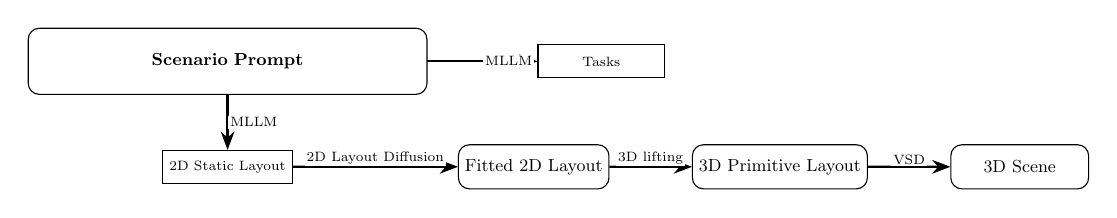
\begin{tikzpicture}[>=Stealth, node distance=0.6cm and 1cm, scale=0.7, transform shape]
  % Styles
  \tikzset{
    block/.style={rectangle, draw, rounded corners, align=center,
      minimum width=2.5cm, minimum height=0.8cm, font=\small},
    sub/.style={rectangle, draw, align=center,
      minimum width=2.3cm, minimum height=0.6cm, font=\scriptsize},
    arrow/.style={-Stealth, thick},
    panel/.style={draw,dashed, rounded corners, inner sep=0.2cm}
  }

  % ----- Panel (a): Input and Splitting -----
  \node[block, minimum height=1.2cm, text width=7cm, align=center] (input) {%
    \textbf{Scenario Prompt} \\[2pt]
  };

  % Three outputs below input
  \node[sub, below=1cm of input] (p2) {2D Static Layout};
  \node[sub, right=2cm of input] (p4) {Tasks};

  % ----- Panel (b): Static Scene Generator -----
  \node[block, right=3cm of p2] (c1) {Fitted 2D Layout};
  \node[block, right=1.5cm of c1] (c2) {3D Primitive Layout};
  \node[block, right=1.5cm of c2] (c3) {3D Scene};

  % ----- Arrows -----
  \draw[arrow] (input.south) -- node[right, font=\scriptsize, fill=white, inner sep=1pt] {MLLM} (p2.north);
  \draw[arrow] (input.east) -- node[right, font=\scriptsize, fill=white, inner sep=1pt] {MLLM} (p4.west);
  \draw[arrow] (p2.east) -- node[above, font=\scriptsize, fill=white, inner sep=1pt] {2D Layout Diffusion} (c1.west);
  \draw[arrow] (c1.east) -- node[above, font=\scriptsize, fill=white, inner sep=1pt] {3D lifting} (c2.west);
  \draw[arrow] (c2.east) -- node[above, font=\scriptsize, fill=white, inner sep=1pt] {VSD} (c3.west);

  % ----- Images below corresponding boxes -----
  %\node[left=0.4cm of p2] (img2) {\includegraphics[width=2.5cm]{images/gemini_static_example.png}};
  %\node[below=0.4cm of c3] (img1) {\includegraphics[width=2.5cm]{images/scene_example.png}};

\end{tikzpicture}%
}
\caption{Model Architecture}
\label{fig:model_architecture}
\end{figure}


\subsection{Input and Splitting}

Since no existing datasets provide paired text prompts with corresponding urban layouts and tasks, we propose leveraging the capabilities of MLLMs to parse and structure input prompts. Similar approaches have been explored in prior works, such as ChatDyn~\cite{wei2024chatdyn} for action planning, LayoutGPT~\cite{feng2023layoutgpt} for layout generation, and LLM-grounded Diffusion~\cite{lian2023llm} for LLM-conditioned image synthesis.

We first use a multimodal large language model (MLLM) (eg. Gemini) to process the input prompt and split it into the layout and tasks. The classes in the layout are based on the KITTI-360~\cite{liao2022kitti360} dataset. Here is an example of how the input prompt can be split:

\begin{tcolorbox}[examplebox, title=Scene Specification Format]

\textbf{Prompt}:

You are an urban scenario planning assistant. For the following urban scene prompt:\\

\emph{[Urban scene description]}

\vspace{1em}
\noindent Generate a JSON object containing the following fields:
\begin{itemize}
    \item \textbf{static\_layout:} \\
    A $500 \times 500$ 2D layout map represented as an array of objects. Each object must include:
    \begin{itemize}
        \item \texttt{id}: unique identifier
        \item \texttt{type}: one of \{\texttt{pole}, \texttt{traffic sign}, \texttt{smallpole}, \texttt{lamp}, \texttt{trash bin}, \texttt{ground}, \texttt{road}, \texttt{sidewalk}, \texttt{parking}, \texttt{building}, \texttt{garage}, \texttt{fence}, \texttt{gate}, \texttt{vegetation}, \texttt{terrain}, \texttt{rail track}, \texttt{wall}, \texttt{box}, \texttt{vending machine}, \texttt{traffic light}, \texttt{rider}, \texttt{bicycle}, \texttt{motorcycle}, \texttt{motorbike}, \texttt{car}, \texttt{truck}, \texttt{bus}, \texttt{van}, \texttt{trailer}, \texttt{caravan}, \texttt{person}\}
        \item \texttt{position}: $(x, y)$ coordinates in meters within the 2D plane
        \item \texttt{orientation}: angle in degrees (0--360)
        \item \texttt{size}: width and height in meters
        \item \texttt{layer}: Layer classification for interactive scenarios. Choose from the default layers: 
        \begin{itemize}
            \item \textbf{Interactive layers:} 
            \begin{itemize}
                \item \texttt{"Container"}: Objects that can contain or hold other items (e.g., trash bins, boxes, bags)
                \item \texttt{"Support"}: Surfaces that can support objects being placed on them (e.g., tables, shelves, building roofs)
                \item \texttt{"Movable"}: Objects that can be moved or picked up (e.g., cars, people, bicycles, small objects)
                \item \texttt{"Interactable"}: Objects users can interact with or activate (e.g., traffic lights, buttons, switches, doors)
            \end{itemize}
            \item \textbf{Navigation layers:}
            \begin{itemize}
                \item \texttt{"Ground"}: Walkable surfaces (e.g., road, sidewalk, parking, ground)
                \item \texttt{"Wall"}: Vertical barriers (e.g., building walls, fences, barriers)
                \item \texttt{"Entryway"}: Passages and access points (e.g., doors, gates, entrances)
            \end{itemize}
            \item \textbf{Environment layers:}
            \begin{itemize}
                \item \texttt{"Light"}: Light sources (e.g., lamps, street lights)
                \item \texttt{"Camera"}: Viewpoints and surveillance (e.g., security cameras)
                \item \texttt{"State\_object"}: Objects with changing states (e.g., animated elements)
                \item \texttt{"Animated"}: Objects with built-in movement (e.g., fountains, flags)
            \end{itemize}
        \end{itemize}
        Use default layers unless scenario requirements need custom combinations.
    \end{itemize}
    \item \textbf{dynamic\_layout:}
    \begin{itemize}
        \item \texttt{trajectories}: Array of dynamic objects representing movement over time. Each object must include:
        \begin{itemize}
            \item \texttt{id}: Unique identifier
            \item \texttt{type}: One of \{\texttt{rider}, \texttt{bicycle}, \texttt{motorcycle}, \texttt{motorbike}, \texttt{car}, \texttt{truck}, \texttt{bus}, \texttt{van}, \texttt{trailer}, \texttt{caravan}, \texttt{person}\}
            \item \texttt{initial\_position}: $(x, y)$ at time = 0
            \item \texttt{trajectory\_description}: Array of states; each state is of the form \{\texttt{"time": t, "position": [x, y]}\} (with $t$ normalized between 0 and 1)
            \item \texttt{layer}: Layer classification (usually \texttt{"Movable"} for dynamic objects)
        \end{itemize}
    \end{itemize}
    \item \textbf{tasks:}\\
    Before creating tasks, review the static\_layout objects above.
    \begin{itemize}
        \item Task targets must reference actual object \texttt{"type"} values in static\_layout.
        \item Ordered list of guided actions for the pedestrian; each task must include:
        \begin{itemize}
            \item \texttt{id}
            \item \texttt{goal}: \{\texttt{type, target, key\_item}\}
            \begin{itemize}
                \item \texttt{type}: One of [\texttt{"get"}, \texttt{"interact"}, \texttt{"interactWith"}, \texttt{"go"}, \texttt{"place\_in"}, \texttt{"place\_on"}] with exact definitions and required object layers:
                \begin{itemize}
                    \item \texttt{"get"}: Target must be \texttt{layer="Movable"}
                    \item \texttt{"interact"/"interactWith"}: Target must be \texttt{layer="Interactable"}
                    \item \texttt{"go"}: Target must be \texttt{layer="Ground"}
                    \item \texttt{"place\_in"}: Target must be \texttt{layer="Container"}
                    \item \texttt{"place\_on"}: Target must be \texttt{layer="Support"}
                \end{itemize}
                \item \texttt{target}: Must match the exact \texttt{"type"} of an existing object in static\_layout with the correct layer.
                \item \texttt{key\_item}: Optional item needed (null if not needed)
            \end{itemize}
            \item \texttt{constraints}: \{\texttt{precedence}, \texttt{evaluation}\}
            \item \texttt{help}: \{\texttt{baseline}, \texttt{target}, \texttt{failure}\}
            \item \texttt{failure\_condition}: \{\texttt{type}, \texttt{item}\}
            \item \texttt{instructions}: \{\texttt{text\_en}, \texttt{text\_fr}\}
            \item \texttt{trigger}: \{\texttt{object\_id}, \texttt{function}\}
        \end{itemize}
    \end{itemize}
\end{itemize}
\vspace{1em}

\textbf{Input Example}: \\

\emph{Afternoon at a three-way intersection with cars parked on the side. Cars arriving from all sides. Agent must yield and check for cars before crossing.}\\


\noindent\textbf{Output Example:}

\textbf{Static layout:}\\
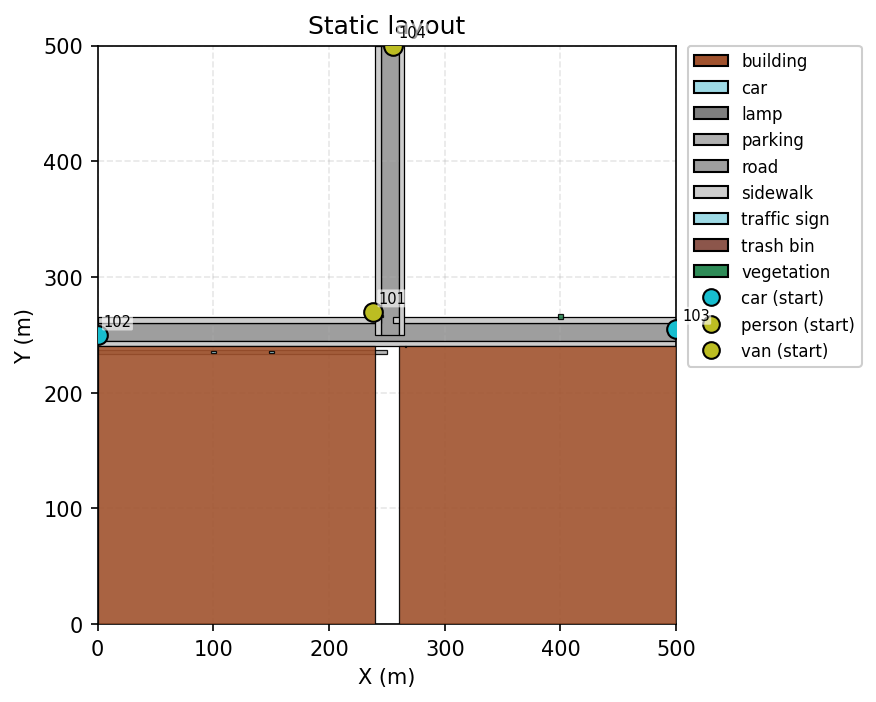
\includegraphics[width=0.8\linewidth]{images/gemini_static.png}


\vspace{1em}

\textbf{Trajectories:}\\
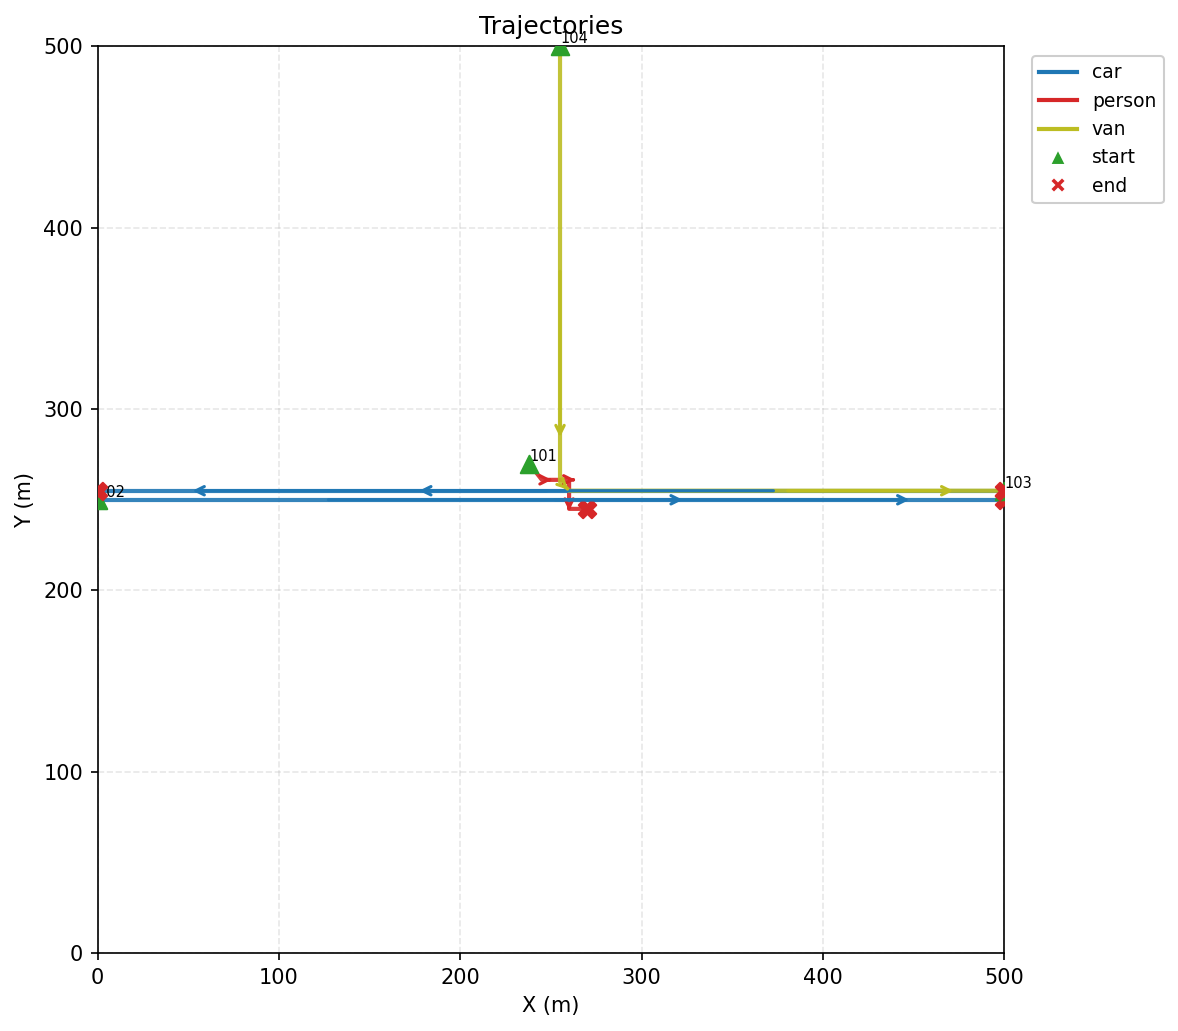
\includegraphics[width=0.8\linewidth]{images/gemini_dynamic.png}



\textbf{Tasks:}
\begin{itemize}[leftmargin=1.2em]
    \item Walk from your starting position at [275, 275] to the edge of the crosswalk at [275, 260].
    \item Wait for the pedestrian signal to allow crossing the horizontal road.
    \item Cross the street to the opposite sidewalk, arriving at [275, 240].
\end{itemize}

JSON for the above available in appendix section~\ref{app:examples:example_json}


\end{tcolorbox}

\subsection{Multinomial Diffusion for Semantic Map Generation}


\begin{tcolorbox}

\textbf{Input example}:

LLM predicted bounding boxes for the prompt: \emph{Road with multiple lanes, guardrails with 2 cars and a truck.}

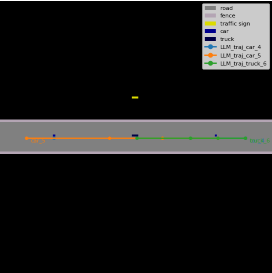
\includegraphics[width=0.6\linewidth]{images/highway_scene_llm.png}

\textbf{Output example}:

The output is a top-down semantic map representing the static elements of the 3D scene to be generated.

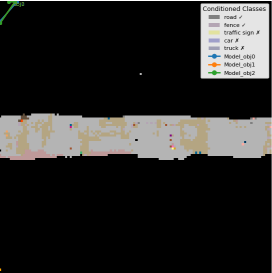
\includegraphics[width=0.6\linewidth]{images/highway_scene_diffusion.png}

\end{tcolorbox}

The next step is to generate a static 3D scene top-down semantic map from the bouding boxes predicted by the MLLM.

\paragraph{1. Preparation of Conditional Inputs}

Given the predicted bounding box layout generated by the MLLM, we build a structured \textit{conditional representation} that serves as the spatial input to the diffusion model. Each bounding box entry in the layout corresponds to a semantic instance (e.g., \textit{road}, \textit{building}, \textit{car}), which is mapped to its corresponding KITTI-360 class ID using a predefined class dictionary.

We then convert the entire layout into a \textit{spatial mask} (conditioning tensor). This process rasterizes all object instances into a dense 2D class map of fixed spatial resolution $(H \times W)$, where each pixel encodes the semantic label of the corresponding region. The result is a tensor 
\[
\mathbf{M} \in \mathbb{R}^{1 \times H \times W},
\]
representing the input condition for the diffusion process.

If dynamic agents and their motion trajectories are available from the MLLM output, we additionally construct a \textit{trajectory tensor} 
\[
\mathbf{T} \in \mathbb{R}^{1 \times N_{\text{dyn}} \times T \times 2},
\]
where $N_{\text{dyn}}$ denotes the number of moving entities and $T$ the number of timesteps. Each trajectory consists of normalized coordinates in map space, which are projected into pixel coordinates consistent with the spatial mask dimensions. To ensure temporal alignment, all trajectories are padded or truncated to a uniform sequence length.

These conditional inputs—the \textbf{semantic spatial mask} and, the \textbf{dynamic trajectory tensor}—form the conditioning context for the diffusion model’s generative process.


\paragraph{2. Multinomial Diffusion for Layout Synthesis.}

Based on the discrete diffusion framework introduced in~\cite{hoogeboom2021argmax}, we design a multinomial diffusion model for semantic layout synthesis. The model uses a U-Net that iteratively denoises top-down semantic maps from the KITTI-360 dataset, conditioned on both static spatial masks and dynamic trajectories. This formulation enables the joint modeling of scene semantics and motion priors.

\paragraph{Forward (noising) process.}
Let $\mathbf{x}_0 \in \{1,\ldots,K\}^{H\times W}$ denote the clean semantic layout, where each pixel corresponds to one of $K$ semantic categories. The forward diffusion process gradually corrupts $\mathbf{x}_0$ through a sequence of categorical random variables $\{\mathbf{x}_t\}_{t=1}^T$ sampled via a fixed multinomial transition kernel:
\begin{equation}
    q(\mathbf{x}_t \mid \mathbf{x}_{t-1}) = \mathrm{Cat}\!\left(
        \mathbf{x}_t ;\,
        (1 - \beta_t)\,\mathbf{1}_{\mathbf{x}_{t-1}} + \beta_t\,\frac{\mathbf{1}}{K}
    \right),
\end{equation}
where $\beta_t \in [0,1]$ denotes the noise schedule and $\mathbf{1}_{\mathbf{x}_{t-1}}$ is the one-hot encoding of $\mathbf{x}_{t-1}$. Repeated application of this transition progressively replaces class labels with uniform noise, such that at step $T$ the distribution approaches:
\begin{equation}
    q(\mathbf{x}_T \mid \mathbf{x}_0) = \mathrm{Cat}\!\left(
        \mathbf{x}_T;\,
        \bar{\alpha}_T\,\mathbf{1}_{\mathbf{x}_0} + (1 - \bar{\alpha}_T)\,\frac{\mathbf{1}}{K}
    \right),
\end{equation}
where $\bar{\alpha}_T = \prod_{s=1}^T (1 - \beta_s)$.

\paragraph{Reverse (denoising) process.}
The reverse process reconstructs $\mathbf{x}_0$ from $\mathbf{x}_T$ by learning the posterior distribution
\begin{equation}
    p_\theta(\mathbf{x}_{t-1} \mid \mathbf{x}_t, \mathbf{c}) =
    \mathrm{Cat}\!\left(
        \mathbf{x}_{t-1};\, \mathbf{p}_\theta(\mathbf{x}_{t-1} \mid \mathbf{x}_t, \mathbf{c})
    \right),
\end{equation}
where $\mathbf{c}$ represents all conditioning inputs (see below).  
At each timestep $t$, the U-Net predicts categorical logits $\mathbf{h}_t$ conditioned on the noisy input, timestep embedding, spatial mask, and motion features:
\begin{align}
    \mathbf{h}_t &= f_\theta(\mathbf{x}_t,\, t,\, \mathbf{M},\, \mathbf{T}),\\
    \mathbf{p}_\theta(\mathbf{x}_{t-1} \mid \mathbf{x}_t, \mathbf{c}) &= \mathrm{softmax}(\mathbf{h}_t).
\end{align}

\paragraph{Training objective and bits-per-dimension.}
The model is trained by minimizing the evidence lower bound (ELBO), which corresponds to the expected cross-entropy between the predicted denoised distribution and the true posterior:
\begin{equation}
    \mathcal{L}_{\text{ELBO}} =
    \sum_{t=1}^T
    \mathbb{E}_{q(\mathbf{x}_t, \mathbf{x}_0)}\!\left[
        \mathrm{KL}\!\left(
        q(\mathbf{x}_{t-1}\mid\mathbf{x}_t,\mathbf{x}_0)
        \,\|\, 
        p_\theta(\mathbf{x}_{t-1}\mid\mathbf{x}_t,\mathbf{c})
        \right)
    \right].
\end{equation}
This objective is implemented as a per-pixel cross-entropy loss.  
To measure log-likelihood quality, we report the ELBO in \textit{bits-per-dimension (bpd)}:
\begin{equation}
    \mathrm{bpd} = 
    \frac{\mathcal{L}_{\text{ELBO}}}{H \times W \times \log 2},
\end{equation}
where lower bpd values indicate higher likelihood and better generative quality.


% \paragraph{Auxiliary trajectory loss.}
% An auxiliary regression head predicts agent trajectories:
% \begin{equation}
%     \mathcal{L}_{\text{traj}} =
%     \mathbb{E}\!\left[
%         \|\widehat{\mathbf{T}}_{\text{refined}} - \mathbf{T}_{\text{gt}}\|_2^2
%     \right],
% \end{equation}
% and the total objective combines both terms:
% \begin{equation}
%     \mathcal{L}_{\text{total}} =
%     \mathcal{L}_{\text{ELBO}} + \lambda_{\text{traj}}\,\mathcal{L}_{\text{traj}},
% \end{equation}
% where $\lambda_{\text{traj}}$ balances static layout reconstruction and trajectory prediction.

\paragraph{Sampling.}
During inference, we begin from a uniform categorical noise map $\mathbf{x}_T$ and iteratively sample
\[
    \mathbf{x}_{t-1} \sim p_\theta(\mathbf{x}_{t-1}\mid \mathbf{x}_t, \mathbf{c}), \quad
    t = T, \ldots, 1,
\]
to produce a semantic layout consistent with the MLLM-generated layout.

\paragraph{Conditioning inputs to the U-Net.}
At each denoising step, the U-Net receives:
\begin{itemize}
  \item \textbf{Noisy semantic map:} $\mathbf{x}_t \in \{0,\ldots,K{-}1\}^{B\times H\times W}$, embedded into a continuous feature space of dimension $d$;
  \item \textbf{Temporal embedding:} a sinusoidal timestep embedding $\tau(t)\in\mathbb{R}^d$, injected into each ResNet block;
  \item \textbf{Static spatial conditioning:} a semantic mask $\mathbf{M}\in\{0,\dots,K{-}1\}^{B\times H_s\times W_s}$ projected via
  \[
    \Phi_{\text{spatial}}:\mathbb{R}^{B\times K\times H_s\times W_s} \to \mathbb{R}^{B\times d\times H\times W};
  \]
  \item \textbf{Dynamic conditioning:} Trajectories 
  $\mathbf{T}_{\text{in}}\in\mathbb{R}^{B\times N_{\text{dyn}}\times T_{\text{in}}\times 2}$ encoded into:
  \begin{align*}
    \mathbf{E}_{\text{obj}} &\in \mathbb{R}^{B\times N_{\text{dyn}}\times d}, &
    \mathbf{e}_{\text{motion}} &\in \mathbb{R}^{B\times d},
  \end{align*}
  where $\mathbf{e}_{\text{motion}}$ modulates U-Net blocks and $\mathbf{E}_{\text{obj}}$ is used by a shared MLP for auxiliary trajectory prediction.
\end{itemize}

\paragraph{Network outputs.}
The U-Net produces:
\begin{itemize}
  \item \textbf{Per-pixel logits:} $\mathrm{logits}\in\mathbb{R}^{B\times K\times H\times W}$ representing categorical distributions for denoising;
  \item \textbf{Auxiliary trajectory predictions:}
  $\widehat{\mathbf{T}}_{\text{refined}}\in\mathbb{R}^{B\times N_{\text{dyn}}\times M\times 2}$, predicted via a shared MLP.
\end{itemize}

\begin{figure}[t]
\centering
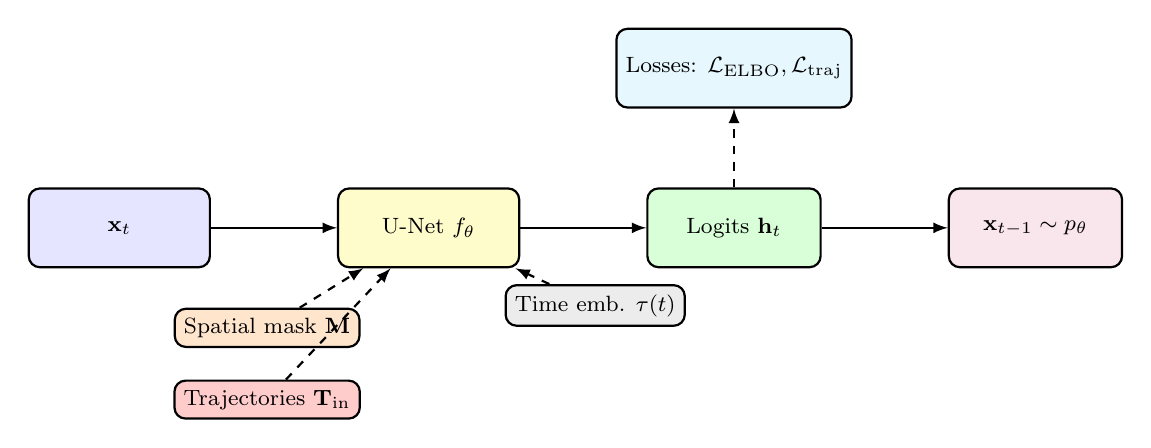
\begin{tikzpicture}[node distance=1.6cm, font=\footnotesize, >=latex, thick]

% Encoder blocks
\node[draw, fill=blue!10, rounded corners, minimum width=2.3cm, minimum height=1cm] (xt) {$\mathbf{x}_t$};
\node[draw, fill=yellow!20, rounded corners, minimum width=2.3cm, minimum height=1cm, right=of xt] (unet) {U-Net $f_\theta$};
\node[draw, fill=green!15, rounded corners, minimum width=2.2cm, minimum height=1cm, right=of unet] (logits) {Logits $\mathbf{h}_t$};
\node[draw, fill=purple!10, rounded corners, minimum width=2.2cm, minimum height=1cm, right=of logits] (sample) {$\mathbf{x}_{t-1}\sim p_\theta$};

% Conditioning inputs
\node[draw, fill=orange!20, rounded corners, below left=0.5cm and -0.3cm of unet] (mask) {Spatial mask $\mathbf{M}$};
\node[draw, fill=red!20, rounded corners, below=0.4cm of mask] (traj) {Trajectories $\mathbf{T}_{\text{in}}$};
\node[draw, fill=gray!15, rounded corners, below right=0.2cm and -0.2cm of unet] (time) {Time emb. $\tau(t)$};

% Arrows
\draw[->] (xt) -- (unet);
\draw[->] (unet) -- (logits);
\draw[->] (logits) -- (sample);
\draw[->, dashed] (mask) -- (unet);
\draw[->, dashed] (traj) -- (unet);
\draw[->, dashed] (time) -- (unet);

% Losses
\node[draw, fill=cyan!10, rounded corners, minimum width=2.5cm, minimum height=1cm, above=1cm of logits] (loss) {Losses: $\mathcal{L}_{\text{ELBO}}, \mathcal{L}_{\text{traj}}$};
\draw[->, dashed] (logits.north) -- (loss.south);

\end{tikzpicture}
\caption{Overview of the multinomial diffusion U-Net for layout synthesis. The model denoises categorical maps $\mathbf{x}_t$ conditioned on spatial and dynamic inputs, optimizing ELBO and auxiliary trajectory losses.}
\label{fig:multinomial_diffusion_arch}
\end{figure}


\paragraph{3. Output}
The final output is a top-down semantic map representing the static elements of the 3D scene to be generated. This map can then be used with score distillation sampling (as shown in Urban Architect~\cite{lu2024urban}) to create the full 3D scene.


\subsection{Tasks}

The tasks predicted by the MLLM are a sequence of guided actions to be performed by the player or agent in the environment. Each task is defined as a structured object, similar to the following JSON format:

\begin{itemize}
    \item \textbf{id:} a unique identifier for the task.
    
    \item \textbf{goal:} specifies the type of action, the target object, and optionally a key item needed to perform the action.
    \begin{itemize}
        \item \texttt{type} -- one of the following:
        \begin{itemize}
            \item \texttt{get}: locate and pick up an object (target must have layer ``Movable'').
            \item \texttt{interact}: interact with an object (target must have layer ``Interactable'').
            \item \texttt{interactWith}: interact with a specific object using a key item (target has layer ``Interactable'').
            \item \texttt{go}: navigate to a location (target must have layer ``Ground'').
            \item \texttt{place\_in}: place an object inside a container (target has layer ``Container'', requires \texttt{key\_item}).
            \item \texttt{place\_on}: place an object on a support surface (target has layer ``Support'', requires \texttt{key\_item}).
        \end{itemize}
        \item \texttt{target} -- the identifier of the target object, using the GUST annotation format:
        \begin{itemize}
            \item Ground objects (layer ``Ground''): \texttt{objecttype\_x.0\_y.0}, e.g., \texttt{sidewalk\_50.0\_62.0}, \texttt{road\_50.0\_50.0}.
            \item Other objects: \texttt{objecttype\_id}, e.g., \texttt{traffic\_light\_4}, \texttt{table\_6}, \texttt{flower\_pot\_8}.
        \end{itemize}
        \item \texttt{key\_item} -- optional object required to perform the task (null for simple tasks, required for \texttt{place\_in}, \texttt{place\_on}, and \texttt{interactWith} tasks).
    \end{itemize}
    
    \item \textbf{baselineTime:} time in seconds that a baseline user should take to complete the task (typically 10--30 seconds for simple tasks, 30--60 seconds for complex tasks).
    
    \item \textbf{targetTime:} maximum time in seconds allowed for the user to complete the task (typically 1.5--2× \texttt{baselineTime}).
    
    \item \textbf{Help system:} provides progressive assistance to the user at different stages.
    \begin{itemize}
        \item \texttt{baselineHelp}: type of help provided after \texttt{baselineTime} elapses (``text'', ``path'', or ``nothing'').
        \item \texttt{targetHelp}: type of help provided after \texttt{targetTime} elapses (``text'', ``path'', or ``nothing'').
        \item \texttt{failureHelp}: type of help provided after task failure (``text'', ``path'', or ``nothing'').
        \item \texttt{baselineText}: English help text shown after \texttt{baselineTime} (e.g., ``Walk straight along the sidewalk'').
        \item \texttt{targetText}: English help text shown after \texttt{targetTime} (e.g., ``Reach the sidewalk safely'').
        \item \texttt{failureText}: English help text shown after failure (e.g., ``Stay on designated walking areas'').
    \end{itemize}
    
    \item \textbf{Failure conditions:} defines when and how the task fails.
    \begin{itemize}
        \item \texttt{failure}: type of failure condition (``collision'' or ``none'').
        \item \texttt{failureItem}: object that causes failure when collided with (e.g., ``vehicle'', ``person''; null if \texttt{failure} is ``none'').
    \end{itemize}
    
    \item \textbf{constraints:} includes task ordering and evaluation criteria.
    \begin{itemize}
        \item \texttt{precedence}: list of task IDs that must be completed before this task can begin.
        \item \texttt{evaluation}: condition that defines successful task completion (e.g., ``on\_sidewalk'', ``item\_picked\_up'').
    \end{itemize}
    
    \item \textbf{instructions:} natural language instructions for the player in multiple languages.
    \begin{itemize}
        \item \texttt{text\_en}: English instructions (e.g., ``Walk to the sidewalk at position [50, 62]'').
        \item \texttt{text\_fr}: French instructions (e.g., ``Marchez vers le trottoir à la position [50, 62]'').
    \end{itemize}
    
    \item \textbf{trigger:} specifies the object and function that triggers task completion.
    \begin{itemize}
        \item \texttt{object\_id}: ID of the object from \texttt{static\_layout}.
        \item \texttt{function}: trigger function name (e.g., ``on\_reach'', ``on\_interact'', ``on\_pickup'').
    \end{itemize}
\end{itemize}

The structure is based on the existing GUsT-3D framework~\cite{wu2022designing} and is integrated with the existing system to provide guided task execution with real-time feedback and progressive assistance.

\section{Evaluation}

For our experiments, we use Gemini 2.5 Flash, Gemini 2.5 Pro and Instruct-VLM as the MLLMs to generate the 3D scene layouts and tasks based on user prompts. We use the KITTI-360 dataset~\cite{liao2022kitti360} to train our multinomial diffusion model for refining the LLM generated semantic maps and trajectories.

\subsection{Prompts}

Based on existing SOTA in prompt engineering, we assess the MLLM along two complementary axes: prompt specificity and scenario plausibility. This framework is informed by SOTA practices in which prompts are structured to test the model across a spectrum of detail starting from vague to detailed, structured guideline (rubric).

\begin{itemize}
    \item \textbf{Prompt specificity:} Measures the model's robustness to variations in instruction detail~\cite{murugadoss2025evaluating, xu2025large}.
    \begin{itemize}
        \item \emph{Vague prompts:} Underspecified instructions for generating urban scenarios, where the model must infer missing details such as city layout, traffic patterns, or population distribution. For example, "Generate an urban scenario with streets and buildings" leaves most design aspects open to the model.
        
        \item \emph{Criteria Specific prompts:} Prompts that specify the desired properties or evaluation criteria for the urban scenario, without detailing exact layouts or steps. For instance, "Generate an urban scenario that is realistic, has safe traffic flow, and includes diverse building types" guides the model toward satisfying these properties while leaving implementation and arrangement open.
        
        \item \emph{Detailed prompts (Rubric):} Fully specified instructions with explicit objectives, constraints, and optional step-by-step guidance for urban scene generation. This may include a rubric enumerating required features, such as "Generate an urban scenario with at least three traffic intersections with controlled signals, a sidewalk along the road and a crosswalk every 50 metres, and pedestrian pathways connecting all major areas. Agent arrives from the north, presses on the pedestrian light and then crosses the road when green." Optional Chain-of-Thought instructions can guide stepwise reasoning for layout design.
    \end{itemize}
    
    \item \textbf{Scenario plausibility:} Evaluates the realism, logical coherence, and potential risk of the model-generated tasks~\cite{parmar2024logicbench, zhu2023promptbench}.
    \begin{itemize}
        \item \emph{Illogical scenarios:} Contain contradictory or impossible instructions to probe reasoning limitations . Example, "Create a scenario with no roads with busy traffic. Agent must cross using the crosswalk."
        \item \emph{Realistic scenarios:} Plausible, safe instructions representing typical interactions. Example, "Create a scenario with multiple cars and bicycles. Agent must wait for the pedestrian signal before crossing."
        \item \emph{Critical scenarios:} Edge-case or high-risk tasks revealing latent model limitations. Example, Jaywalking, Parking lot navigation, etc.
        \item \emph{Prompts reflecting original GUsT-3D scenarios:} Baseline scenarios sourced directly from the dataset for comparison with prior work.
    \end{itemize}
\end{itemize}

\paragraph{Prompt Grid Design}  
To systematically explore model behavior, each task is tested using prompts that span the two axes. Conceptually, this forms a 2D evaluation grid:

\begin{center}
\begin{tabular}{c|c|c|c}
\textbf{Prompt Specificity} & \textbf{Illogical} & \textbf{Realistic} & \textbf{Critical} \\ \hline
\textbf{Vague} & P1 & P2 & P3 \\
\textbf{Detailed} & P4 & P5 & P6
\end{tabular}
\end{center}

Here, P1--P6 represent prompts designed for each combination of specificity and scenario plausibility.

\subsection{Quantitative Evaluation}

To quantitatively evaluate the quality of the generated 3D scenarios, we propose the following metrics:

TODO

\section{Implementation}

The implementation of the system is divided into two components — the \textbf{Backend (Python)} and the \textbf{Frontend (Unity)} — which together enable interaction between the MLLM (Gemini 2.5 pro for our case), the multinomial diffusion model and the Unity-based scenario generation environment.

\subsection{Backend (Python) Implementation}

The backend is implemented as an HTTP server in Python that interfaces with various MLLMs to process requests and manage data flow between the model and the Unity client. 
It exposes four primary \texttt{POST} endpoints:

\begin{itemize}
    \item \textbf{/get\_json} – Generates the initial layout or configuration in JSON format based on user input or scene specifications.
    \item \textbf{/refine\_layout} – Refines the generated layout using the multinomial diffusion model.
    \item \textbf{/get\_3d} – Produces 3D representations or assets produuced by Urban Architect~\cite{lu2024urban}.
    \item \textbf{/get\_tasks} – Provides task-level metadata or scenario instructions to GUsT-3D
\end{itemize}

\subsection{Frontend (Unity) Implementation}

The frontend is developed as a part of existing GUsT-3D add-on. It communicates with the Python backend via HTTP, sending requests to the defined endpoints and parsing the responses to generate the scenarios within Unity.


\section{Experiments}
\label{sec:experiments}

This section presents a log of all experiments conducted to train the \textit{multinomial diffusion model}. Detailed parameters of the experiments are available in \emph{attachments/runs.csv} for reference. Table~\ref{tab:validation_results} visualises the validation results for each experiment, whereas Table~\ref{tab:llm_results} visualises the LLM conditioning results for each experiment. Figure~\ref{fig:legend} shows the legend of the generated maps.

\subsection{Experiment 1: \texttt{notebook\_test}}

\textbf{Goal:} Train the model based on the degraded semantic maps extracted from the KITTI-360 layouts.

\textbf{Parameters:}
\begin{itemize}
    \item Latent Dimension: 32
    \item Timesteps: 100
    \item Epochs: 100
    \item Number of maps: 100
\end{itemize}


\textbf{Results:}
\begin{itemize}
    \item The losses oscillated significantly due to a high learning rate as shown in Figure~\ref{fig:loss_curves_ep1}.
    \item Training failed.
\end{itemize}


\begin{figure}
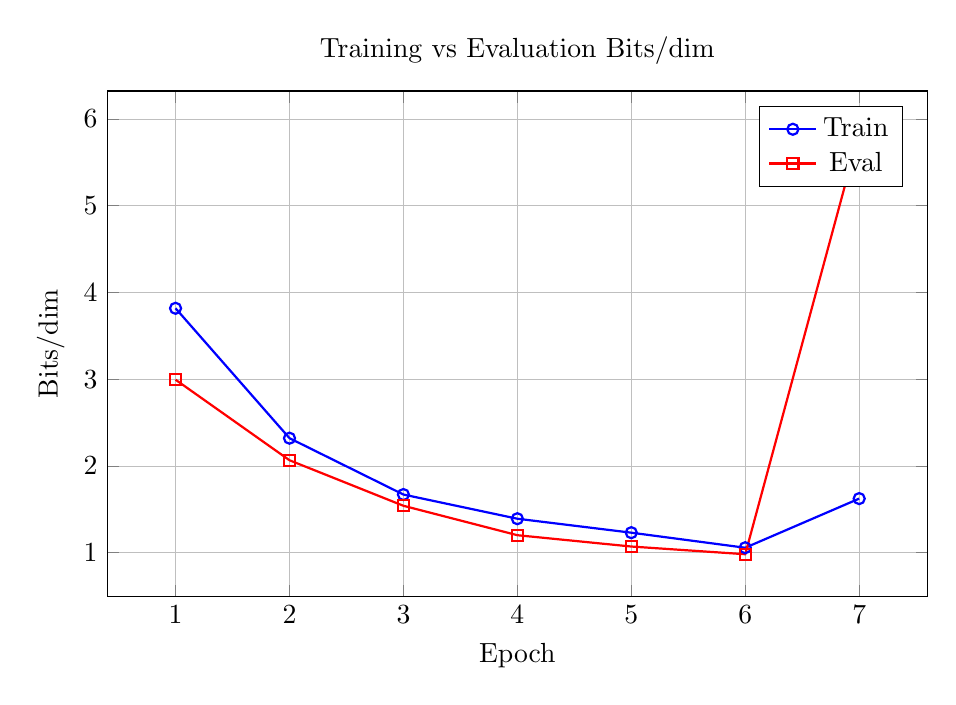
\begin{tikzpicture}
\begin{axis}[
    width=12cm,
    height=8cm,
    xlabel={Epoch},
    ylabel={Bits/dim},
    title={Training vs Evaluation Bits/dim},
    legend pos=north east,
    grid=both,
    major grid style={line width=0.2pt,draw=gray!50},
    minor grid style={line width=0.1pt,draw=gray!20},
]

% Training curve
\addplot[
    color=blue,
    mark=o,
    thick,
] coordinates {
  (1, 3.81698)
  (2, 2.31937)
  (3, 1.66945)
  (4, 1.39065)
  (5, 1.2297)
  (6, 1.05613)
  (7, 1.62261)
  (8, nan)
  (9, nan)
  (10, nan)
  (11, nan)
  (12, nan)
  (13, nan)
  (14, nan)
  (15, nan)
  (16, nan)
};
\addlegendentry{Train}

% Evaluation curve
\addplot[
    color=red,
    mark=square,
    thick,
] coordinates {
  (1, 2.99358)
  (2, 2.06491)
  (3, 1.53996)
  (4, 1.20063)
  (5, 1.07013)
  (6, 0.98127)
  (7, 5.83726)
  (8, nan)
  (9, nan)
  (10, nan)
  (11, nan)
  (12, nan)
  (13, nan)
  (14, nan)
  (15, nan)
  (16, nan)
};
\addlegendentry{Eval}
\end{axis}
\end{tikzpicture}
\caption{Loss curves for Experiment 1}
\label{fig:loss_curves_ep1}
\end{figure}


\subsection{Experiment 2: \texttt{notebook\_test\_stable}}

\textbf{Goal:} Based on the previous results. The goal of this run was to stabilise the training as well as check the training and inference for the trajectory generation code.

\textbf{Parameters:}
\begin{itemize}
    \item Class weights: added based for trajectories based on the frequency of dynamic classes.
    \item Latent Dimension: 64
    \item Timesteps: 1000
    \item Number of maps: 15000 
    \item File stride: 5 
    \item Epochs: 50
\end{itemize}


\textbf{Changes Made:}
\begin{itemize}
    \item Decreased learning rate by a factor of 10 for more stable convergence.
    \item Added input augmentations (rotations and flips) to improve dataset variability.
    \item Increased diffusion embedding dimension from 32 to 64 to mitigate class swapping.
    \item Increased diffusion timesteps from 100 to 1000 (improving quality at the cost of training/inference time).
    \item Implemented the following enhancements:
    \begin{itemize}
        \item \textbf{Trajectory logic:} Introduced to handle dynamic elements.
        \item \textbf{Class weights:} Applied to dynamic classes to handle class imbalance.
        \item \textbf{File stride:} Sampling every $n$th file to increase variability.
        \item \textbf{Frame skip:} Similar to stride, but applied to trajectory sequences.
        \item \textbf{Sequence length:} Defined the number of frames per trajectory.
    \end{itemize}
\end{itemize}

\textbf{Results:}
\begin{itemize}
    \item The training became significantly more stable compared to the previous run. The lower validation loss compared to the training loss could be due to a smaller number of epochs. Additionally, the validation loss is measured after each training epoch.  Figure~\ref{fig:loss_curves_ep2} shows the loss curves for each epoch.
    \item The static generation generates artefacts (such as the dynamic components) as shown in tables~\ref{tab:validation_results} and~\ref{tab:llm_results}.
    \item The trajectory tensors had much lower values and didn't conform to the spatial mask.
\end{itemize}

\begin{figure}
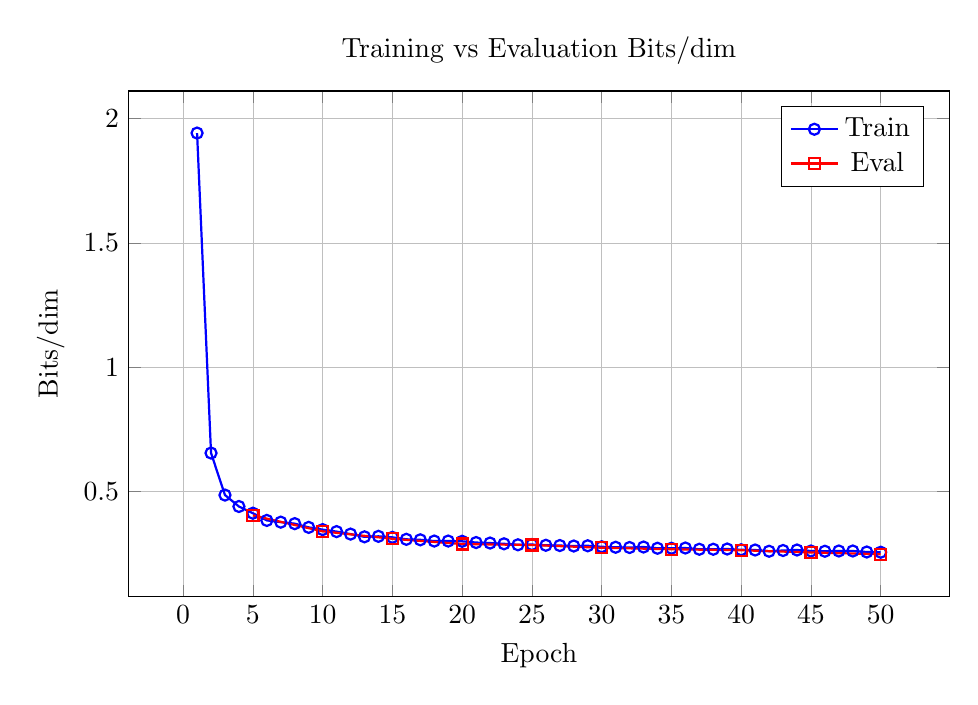
\begin{tikzpicture}
\begin{axis}[
    width=12cm,
    height=8cm,
    xlabel={Epoch},
    ylabel={Bits/dim},
    title={Training vs Evaluation Bits/dim},
    legend pos=north east,
    grid=both,
    major grid style={line width=0.2pt,draw=gray!50},
    minor grid style={line width=0.1pt,draw=gray!20},
]

% Training curve
\addplot[
    color=blue,
    mark=o,
    thick,
] coordinates {
(1,1.942)
(2,0.655)
(3,0.486)
(4,0.440)
(5,0.413)
(6,0.384)
(7,0.377)
(8,0.371)
(9,0.356)
(10,0.347)
(11,0.339)
(12,0.329)
(13,0.318)
(14,0.320)
(15,0.316)
(16,0.308)
(17,0.306)
(18,0.301)
(19,0.301)
(20,0.300)
(21,0.295)
(22,0.293)
(23,0.290)
(24,0.286)
(25,0.287)
(26,0.284)
(27,0.283)
(28,0.281)
(29,0.282)
(30,0.278)
(31,0.276)
(32,0.275)
(33,0.277)
(34,0.272)
(35,0.272)
(36,0.273)
(37,0.268)
(38,0.268)
(39,0.269)
(40,0.266)
(41,0.265)
(42,0.260)
(43,0.263)
(44,0.265)
(45,0.261)
(46,0.260)
(47,0.261)
(48,0.261)
(49,0.257)
(50,0.256)
};
\addlegendentry{Train}

% Evaluation curve
\addplot[
    color=red,
    mark=square,
    thick,
] coordinates {
(5,0.404)
(10,0.340)
(15,0.310)
(20,0.289)
(25,0.285)
(30,0.274)
(35,0.268)
(40,0.264)
(45,0.255)
(50,0.248)
};
\addlegendentry{Eval}
\end{axis}
\end{tikzpicture}
\caption{Loss curves for Experiment 2}
\label{fig:loss_curves_ep2}
\end{figure}

% \begin{figure}
%     \centering
%     \includegraphics[width=0.8\textwidth]{images/trajectory_results_val_exp2.png}
%     \captionof{figure}{Trajectory results on validation samples. Left: KITTI-360 ground truth. Middle: Diffusion model output. Right: LLM-generated map used as conditioning.}
%     \label{fig:trajectory_results_val_exp2}
% \end{figure}

% \begin{figure}
%     \centering
%     \includegraphics[width=0.8\textwidth]{images/trajectory_results_llm_exp2.png}
%     \captionof{figure}{Trajectory results on LLM-generated samples.}
%     \label{fig:trajectory_results_llm_exp2}
% \end{figure}


\subsection{Experiment 3: \texttt{run\_20251023\_020445}}

\textbf{Goal:} Conduct a complete static layout generation run after incorporating insights from prior experiments and discussions.

\textbf{Changes Made:}
\begin{itemize}
    \item Ignored class weights and trajectory-related computations to focus solely on static layout generation.
    \item Replaced bounding-box extraction with a grid-based approach to convert exact shape masks into bounding boxes. This approach aligns better with the blocky, large-object nature of LLM-generated outputs.
\end{itemize}

\textbf{Parameters:}
\begin{itemize}
    \item Class weights: added based for trajectories based on the frequency of dynamic classes.
    \item Latent Dimension: 64
    \item Timesteps: 1000
    \item Number of maps: 7500 
    \item File stride: 10
    \item Epochs: 25
\end{itemize}


\textbf{Results:}
\begin{enumerate}
    \item Final training and validation loss of 0.25 and 0.24. The training and validation loss curves are shown in Figure~\ref{fig:loss_curves_ep4}.

    \item The model does regenerate the main structures in the images, but it also introduces dynamic objects, such as cars, into the static map. Figure~\ref{fig:legend} shows the legend of the generated maps. In future, A better approach could be to mask out these dynamic objects completely from the training data for static inference.
\end{enumerate}

\begin{figure}
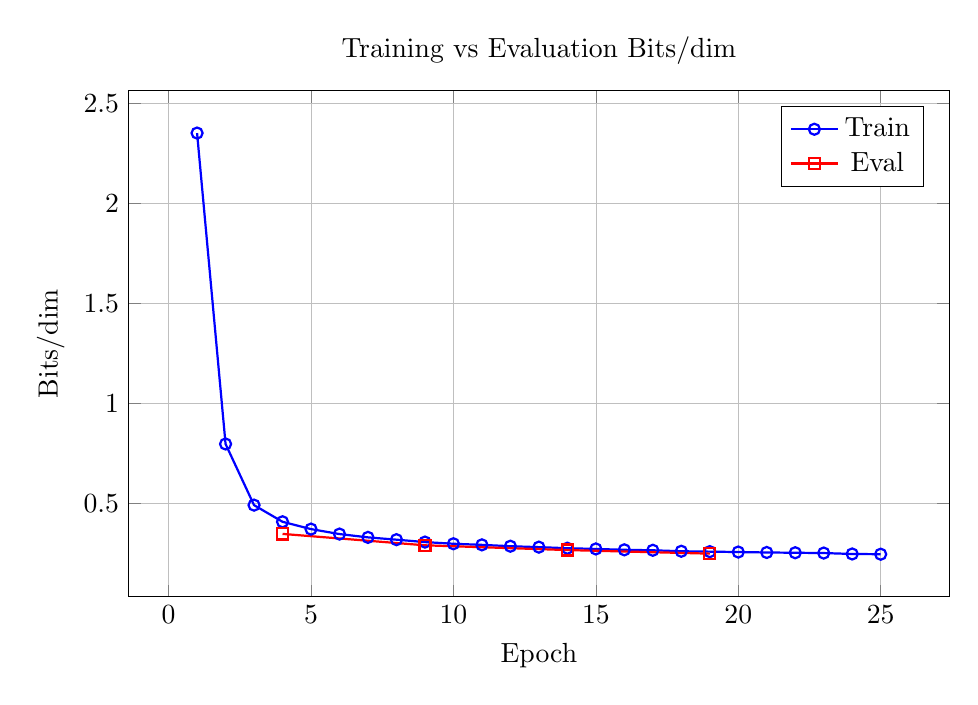
\begin{tikzpicture}
\begin{axis}[
    width=12cm,
    height=8cm,
    xlabel={Epoch},
    ylabel={Bits/dim},
    title={Training vs Evaluation Bits/dim},
    legend pos=north east,
    grid=both,
    major grid style={line width=0.2pt,draw=gray!50},
    minor grid style={line width=0.1pt,draw=gray!20},
]

% Training curve
\addplot[
    color=blue,
    mark=o,
    thick,
] coordinates {
(1,2.3510)
(2,0.7959)
(3,0.4901)
(4,0.4068)
(5,0.3702)
(6,0.3454)
(7,0.3288)
(8,0.3173)
(9,0.3053)
(10,0.2969)
(11,0.2914)
(12,0.2846)
(13,0.2800)
(14,0.2746)
(15,0.2710)
(16,0.2666)
(17,0.2643)
(18,0.2594)
(19,0.2575)
(20,0.2555)
(21,0.2533)
(22,0.2519)
(23,0.2504)
(24,0.2458)
(25,0.2446)
};
\addlegendentry{Train}

% Evaluation curve
\addplot[
    color=red,
    mark=square,
    thick,
] coordinates {
(4,0.3462)
(9,0.28919)
(14,0.26535)
(19,0.24751)
};
\addlegendentry{Eval}
\end{axis}
\end{tikzpicture}
\caption{Loss curves for Experiment 3}
\label{fig:loss_curves_exp3}
\end{figure}


\begin{figure}
    \centering
    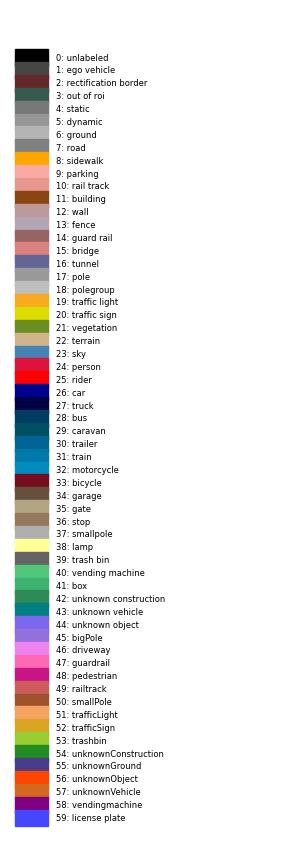
\includegraphics[width=0.4\textwidth]{images/legend.png}
    \captionof{figure}{Legend for generated maps.}
    \label{fig:legend}
\end{figure}


\subsection{Experiment 4: \texttt{run\_20251025\_031240}}

\textbf{Goal:} Conduct a complete static layout generation run after incorporating insights from prior experiments and discussions.

\textbf{Parameters:}
\begin{itemize}
    \item Class weights: added based for trajectories based on the frequency of dynamic classes.
    \item Latent Dimension: 64
    \item Timesteps: 1000
    \item Number of maps: 5000 
    \item File stride: 14
    \item Epochs: 50
\end{itemize}

\textbf{Changes Made:}
\begin{itemize}
    \item Ignored class weights and trajectory-related computations to focus solely on static layout generation.
    \item Replaced bounding-box extraction with a grid-based approach to convert exact shape masks into bounding boxes. This approach aligns better with the blocky, large-object nature of LLM-generated outputs.
\end{itemize}


\textbf{Results:}
\begin{enumerate}
    \item Final training and validation loss of 0.157 and 0.224. An additional test loss of 0.229803 was calculated on the test dataset after the training The training and validation loss curves are shown in Figure~\ref{fig:loss_curves_ep4}. The much-lower training loss in this run suggests that the model overfitted to the training data compared to previous which is also reflected by the increase in validation loss in last 10 epochs.

    \item The model does not introduce dynamic objects, and also infills static objects for certain maps. However, some artefacts are still present in the generated maps as shown in tables~\ref{tab:validation_results} and~\ref{tab:llm_results}.
\end{enumerate}

\begin{figure}
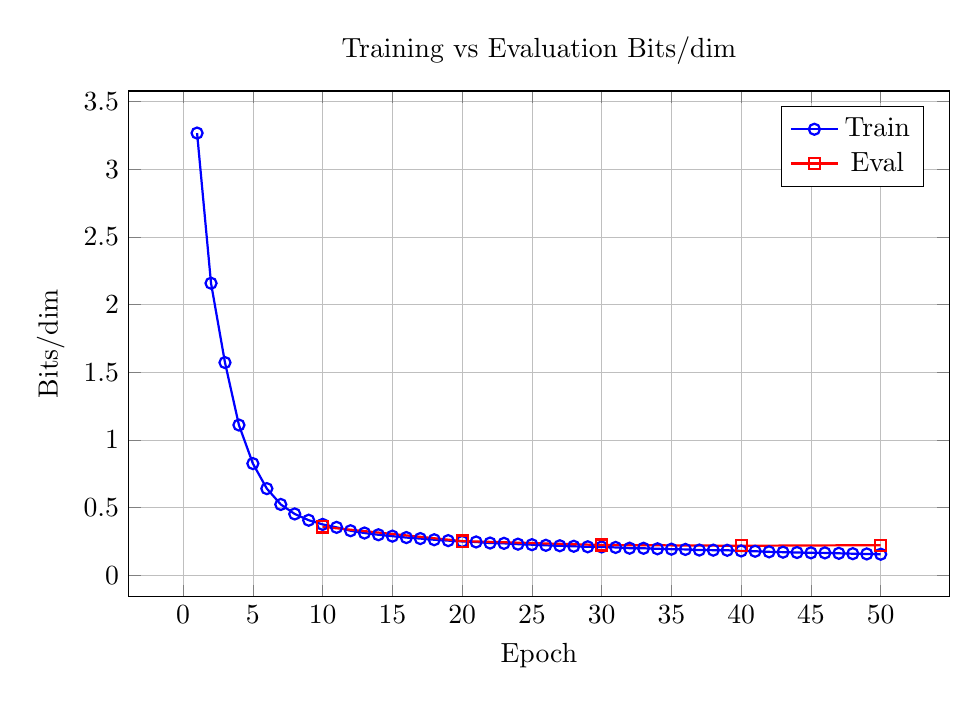
\begin{tikzpicture}
\begin{axis}[
    width=12cm,
    height=8cm,
    xlabel={Epoch},
    ylabel={Bits/dim},
    title={Training vs Evaluation Bits/dim},
    legend pos=north east,
    grid=both,
    major grid style={line width=0.2pt,draw=gray!50},
    minor grid style={line width=0.1pt,draw=gray!20},
]

% Training curve
\addplot[
    color=blue,
    mark=o,
    thick,
] coordinates {
(1,3.266052022116525 )
(2,2.1576013405663628)
(3,1.5719009031568254)
(4,1.1108483610834394)
(5,0.8262577911104475)
(6,0.6413788035256522)
(7,0.524440433365958 )
(8,0.45429373802457534)
(9,0.4082127619130271)
(10,0.37728283963884623)
(11,0.35537326564107624)
(12,0.3304433267797743)
(13,0.31359455631460464)
(14,0.3008075200830187)
(15,0.2905022528171539)
(16,0.28004381128719874)
(17,0.27268179556301664)
(18,0.2640313944816589)
(19,0.25760547358649116)
(20,0.2514811924185072)
(21,0.2475815166405269)
(22,0.23972793780054366)
(23,0.23745073865141186)
(24,0.2313898389339447)
(25,0.22757616998468128)
(26,0.22290931400230954)
(27,0.21951803415162222)
(28,0.21580973981107984)
(29,0.21199409898689814)
(30,0.21082251518113274)
(31,0.20724563092844828)
(32,0.20156505715847015)
(33,0.20100805059501103)
(34,0.19720662110192436)
(35,0.19440724221297673)
(36,0.19261907357828958)
(37,0.18792454389163427)
(38,0.18714307463169097)
(39,0.18626809465885164)
(40,0.1813189321586064)
(41,0.17906540957518988)
(42,0.17472429156303407)
(43,0.1723263396535601)
(44,0.1698573808840343)
(45,0.16727627163273948)
(46,0.16689756722109658)
(47,0.16381815944399153)
(48,0.1610402065856116)
(49,0.1591573236669813)
(50,0.15715532231330873)
};
\addlegendentry{Train}

% Evaluation curve
\addplot[
    color=red,
    mark=square,
    thick,
] coordinates {
(10,0.35908874416351316)
(20,0.25402949523925783)
(30,0.22512340140342713)
(40,0.21949620628356933)
(50,0.2240180037021637)
};
\addlegendentry{Eval}
\end{axis}
\end{tikzpicture}
\caption{Loss curves for Experiment 4}
\label{fig:loss_curves_ep4}
\end{figure}


\subsection{Experiment 5 (planned)}
\textbf{Goal:} Despite lower training and val losses, the generalisation by the diffusion model, especially on LLM maps, still has problems. This is due to the discrepancy in the input of the diffusion and the output of the LLM. The LLM generates the map using a JSON structure that contains larger, continuous objects compared to the pixelated semantic maps, which serve as input conditioning for the diffusion model. The goal of this experiment is to adapt the LLM's output format to the diffusion model's input format to improve generalisation. For this, the VLM has to be finetuned to generate a detailed pixel-wise map inside the JSON structure itself. 

\textbf{Changes to be Made:}
\begin{itemize}
    \item Switch the MLLM used from Gemini (closed-source) to Instruct-VL3 (open-source)
    \item Create synthetic class-to-json pairs of a subset of semantic maps which will be used to finetune the model.
    \item Use QLoRA~\cite{dettmers2023qlora} for finetuning.
    \item For validation, 1000 generaeted samples will be compared using FID, KID, and CKL metrics to measure the distribution distance from the eval set (table~\ref{tab:validation}).
\end{itemize}

\textbf{Results:}
\begin{enumerate}
    \item 
\end{enumerate}

\begin{table}
\centering
\caption{Comparison of Validation Conditioning, Ground Truth, and Inferred Images}
\begin{tabular}{c | c | c}
%\toprule
%\multicolumn{3}{c}{\textbf{Ground Truth}} \\
%\midrule
%\multicolumn{3}{c}{
  %
\includegraphics[width=0.25\linewidth]{images/val_gt1.png} \hspace{2pt}
  %\includegraphics[width=0.25\linewidth]%{images/val_gt2.png} \hspace{2pt}
 % \includegraphics[width=0.25\linewidth]{images/val_gt3.png}
%} \\
%\midrule
\textbf{Exp. No.} & \textbf{Conditioning} & \textbf{Inferred Image} \\
\midrule

1 & \multicolumn{2}{c}{Training Unstable} \\
\midrule

2 &

\includegraphics[width=0.15\linewidth]{images/val_conditioning1_exp2.png}

\includegraphics[width=0.15\linewidth]{images/val_conditioning2_exp2.png}
%\includegraphics[width=0.15\linewidth]{images/val_conditioning3_exp2.png}
&

\includegraphics[width=0.15\linewidth]{images/val_inferred1_exp2.png}

\includegraphics[width=0.15\linewidth]{images/val_inferred2_exp2.png}
%\includegraphics[width=0.15\linewidth]{images/val_inferred3_exp2.png}
\\
\midrule

3 &

\includegraphics[width=0.15\linewidth]{images/val_conditioning1_exp3.png}

\includegraphics[width=0.15\linewidth]{images/val_conditioning2_exp3.png}
%\includegraphics[width=0.15\linewidth]{images/val_conditioning3_exp3.png}
&

\includegraphics[width=0.15\linewidth]{images/val_inferred1_exp3.png}

\includegraphics[width=0.15\linewidth]{images/val_inferred2_exp3.png}
%\includegraphics[width=0.15\linewidth]{images/val_inferred3_exp3.png}
\\
\midrule

4 &

\includegraphics[width=0.15\linewidth]{images/val_conditioning1_exp4.png}

\includegraphics[width=0.15\linewidth]{images/val_conditioning2_exp4.png}
%\includegraphics[width=0.15\linewidth]{images/val_conditioning3_exp4.png} 
&

\includegraphics[width=0.15\linewidth]{images/val_inferred1_exp4.png}

\includegraphics[width=0.15\linewidth]{images/val_inferred2_exp4.png}
%\includegraphics[width=0.15\linewidth]{images/val_inferred3_exp4.png} 
\\

\bottomrule
\end{tabular}
\caption*{Top: Ground truth semantic maps used as conditioning input. Below: The conditionings and inferred outputs from the diffusion model across four experiments.}
\label{tab:validation_results}
\end{table}

\begin{table}
\centering
\caption{Comparison of LLM Conditioning and Inferred Images}
\begin{tabular}{c | c}
\toprule
\multicolumn{2}{c}{\textbf{LLM Conditioning}} \\
\midrule
\multicolumn{2}{c}{
  
\includegraphics[width=0.25\linewidth]{images/llm_conditioning1.png} \hspace{2pt}
  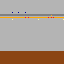
\includegraphics[width=0.25\linewidth]{images/llm_conditioning2.png} \hspace{2pt}
  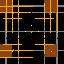
\includegraphics[width=0.25\linewidth]{images/llm_conditioning3.png}
} \\
\midrule
\textbf{Exp. No.} & \textbf{Inferred Image} \\
\midrule

1 & \multicolumn{1}{c}{Training Unstable} \\
\midrule

2 &

\includegraphics[width=0.15\linewidth]{images/llm_inferred1_exp2.png}

\includegraphics[width=0.15\linewidth]{images/llm_inferred2_exp2.png}

\includegraphics[width=0.15\linewidth]{images/llm_inferred3_exp2.png} \\
\midrule

3 &

\includegraphics[width=0.15\linewidth]{images/llm_inferred1_exp3.png}

\includegraphics[width=0.15\linewidth]{images/llm_inferred2_exp3.png}

\includegraphics[width=0.15\linewidth]{images/llm_inferred3_exp3.png} \\
\midrule

4 &

\includegraphics[width=0.15\linewidth]{images/llm_inferred1_exp4.png}

\includegraphics[width=0.15\linewidth]{images/llm_inferred2_exp4.png}

\includegraphics[width=0.15\linewidth]{images/llm_inferred3_exp4.png} \\

\bottomrule
\end{tabular}
\caption*{Top: LLM-generated semantic maps used as conditioning input. Below: Inferred outputs from the diffusion model across four experiments.}
\label{tab:llm_results}
\end{table}


\clearpage
\section*{Appendix}

\section{Examples}

\subsection{Layout JSON}
\label{app:examples:example_json}

\begin{verbatim}
{
  "static_layout": [
    {
      "id": 1,
      "type": "road",
      "position": [
        250,
        250
      ],
      "size": [
        500,
        20
      ],
      "orientation": 0,
      "layer": "Ground"
    },
    {
      "id": 2,
      "type": "road",
      "position": [
        250,
        250
      ],
      "size": [
        20,
        500
      ],
      "orientation": 90,
      "layer": "Ground"
    },
    {
      "id": 3,
      "type": "sidewalk",
      "position": [
        250,
        230
      ],
      "size": [
        500,
        10
      ],
      "orientation": 0,
      "layer": "Ground"
    },
    {
      "id": 4,
      "type": "sidewalk",
      "position": [
        250,
        270
      ],
      "size": [
        500,
        10
      ],
      "orientation": 0,
      "layer": "Ground"
    },
    {
      "id": 5,
      "type": "sidewalk",
      "position": [
        230,
        250
      ],
      "size": [
        10,
        500
      ],
      "orientation": 90,
      "layer": "Ground"
    },
    {
      "id": 6,
      "type": "sidewalk",
      "position": [
        270,
        250
      ],
      "size": [
        10,
        500
      ],
      "orientation": 90,
      "layer": "Ground"
    },
    {
      "id": 7,
      "type": "building",
      "position": [
        50,
        50
      ],
      "size": [
        100,
        100
      ],
      "orientation": 0,
      "layer": "Wall"
    },
    {
      "id": 8,
      "type": "building",
      "position": [
        450,
        50
      ],
      "size": [
        100,
        100
      ],
      "orientation": 0,
      "layer": "Wall"
    },
    {
      "id": 9,
      "type": "building",
      "position": [
        50,
        450
      ],
      "size": [
        100,
        100
      ],
      "orientation": 0,
      "layer": "Wall"
    },
    {
      "id": 10,
      "type": "building",
      "position": [
        450,
        450
      ],
      "size": [
        100,
        100
      ],
      "orientation": 0,
      "layer": "Wall"
    },
    {
      "id": 11,
      "type": "traffic light",
      "position": [
        240,
        220
      ],
      "size": [
        2,
        5
      ],
      "orientation": 0,
      "layer": "Interactable"
    },
    {
      "id": 12,
      "type": "traffic light",
      "position": [
        260,
        280
      ],
      "size": [
        2,
        5
      ],
      "orientation": 180,
      "layer": "Interactable"
    },
    {
      "id": 13,
      "type": "traffic light",
      "position": [
        220,
        260
      ],
      "size": [
        2,
        5
      ],
      "orientation": 270,
      "layer": "Interactable"
    },
    {
      "id": 14,
      "type": "traffic light",
      "position": [
        280,
        240
      ],
      "size": [
        2,
        5
      ],
      "orientation": 90,
      "layer": "Interactable"
    },
    {
      "id": 15,
      "type": "vegetation",
      "position": [
        150,
        150
      ],
      "size": [
        5,
        5
      ],
      "orientation": 0,
      "layer": "Environment"
    },
    {
      "id": 16,
      "type": "vegetation",
      "position": [
        350,
        150
      ],
      "size": [
        5,
        5
      ],
      "orientation": 0,
      "layer": "Environment"
    },
    {
      "id": 17,
      "type": "vegetation",
      "position": [
        150,
        350
      ],
      "size": [
        5,
        5
      ],
      "orientation": 0,
      "layer": "Environment"
    },
    {
      "id": 18,
      "type": "vegetation",
      "position": [
        350,
        350
      ],
      "size": [
        5,
        5
      ],
      "orientation": 0,
      "layer": "Environment"
    },
    {
      "id": 19,
      "type": "ground",
      "position": [
        250,
        250
      ],
      "size": [
        20,
        20
      ],
      "orientation": 0,
      "layer": "Ground"
    }
  ],
  "dynamic_layout": {
    "trajectories": [
      {
        "id": 101,
        "type": "car",
        "initial_position": [
          100,
          250
        ],
        "layer": "Movable",
        "trajectory_description": [
          {
            "time": 0.0,
            "position": [
              100,
              250
            ]
          },
          {
            "time": 0.5,
            "position": [
              250,
              250
            ]
          },
          {
            "time": 0.7,
            "position": [
              250,
              235
            ]
          },
          {
            "time": 0.9,
            "position": [
              265,
              250
            ]
          }
        ]
      },
      {
        "id": 102,
        "type": "car",
        "initial_position": [
          250,
          400
        ],
        "layer": "Movable",
        "trajectory_description": [
          {
            "time": 0.0,
            "position": [
              250,
              400
            ]
          },
          {
            "time": 0.5,
            "position": [
              250,
              250
            ]
          },
          {
            "time": 0.7,
            "position": [
              235,
              250
            ]
          },
          {
            "time": 0.9,
            "position": [
              250,
              265
            ]
          }
        ]
      },
      {
        "id": 103,
        "type": "bicycle",
        "initial_position": [
          300,
          230
        ],
        "layer": "Movable",
        "trajectory_description": [
          {
            "time": 0.0,
            "position": [
              300,
              230
            ]
          },
          {
            "time": 0.3,
            "position": [
              300,
              250
            ]
          },
          {
            "time": 0.6,
            "position": [
              250,
              250
            ]
          },
          {
            "time": 0.8,
            "position": [
              235,
              250
            ]
          }
        ]
      },
      {
        "id": 104,
        "type": "person",
        "initial_position": [
          300,
          215
        ],
        "layer": "Movable",
        "trajectory_description": [
          {
            "time": 0.0,
            "position": [
              300,
              215
            ]
          },
          {
            "time": 0.3,
            "position": [
              300,
              230
            ]
          },
          {
            "time": 0.6,
            "position": [
              300,
              250
            ]
          },
          {
            "time": 0.8,
            "position": [
              300,
              270
            ]
          }
        ]
      }
    ]
  },
  "tasks": [
    {
      "id": 1,
      "goal": {
        "type": "go",
        "target": "sidewalk_300.0_230.0",
        "key_item": null
      },
      "constraints": {
        "precedence": [],
        "evaluation": "arrive_at_target"
      },
      "help": {
        "baseline": "Head towards the sidewalk to wait for the cyclist.",
        "target": "Reach the designated waiting area.",
        "failure": "Do not enter the road until safe."
      },
      "failure_condition": {
        "type": "collision",
        "item": "car"
      },
      "instructions": {
        "text_en": "Go to the sidewalk at [300, 230] and wait.",
        "text_fr": "Allez sur le trottoir \u00e0 [300, 230] et attendez."
      },
      "trigger": {
        "object_id": 3,
        "function": "on_reach"
      }
    },
    {
      "id": 2,
      "goal": {
        "type": "interact",
        "target": "traffic_light_11",
        "key_item": null
      },
      "constraints": {
        "precedence": [
          1
        ],
        "evaluation": "light_green"
      },
      "help": {
        "baseline": "Observe the traffic light and wait for it to turn green.",
        "target": "Wait for the pedestrian signal to be green.",
        "failure": "Crossing on red is dangerous."
      },
      "failure_condition": {
        "type": "violation",
        "item": "traffic_light"
      },
      "instructions": {
        "text_en": "Wait for the traffic light at [240, 220] to turn green before proceeding.",
        "text_fr": "Attendez que le feu de circulation \u00e0 [240, 220] passe au vert."
      },
      "trigger": {
        "object_id": 11,
        "function": "on_light_green"
      }
    },
    {
      "id": 3,
      "goal": {
        "type": "go",
        "target": "road_250.0_250.0",
        "key_item": null
      },
      "constraints": {
        "precedence": [
          2
        ],
        "evaluation": "arrive_at_target"
      },
      "help": {
        "baseline": "Cross the intersection carefully.",
        "target": "Cross the road safely.",
        "failure": "Avoid vehicles."
      },
      "failure_condition": {
        "type": "collision",
        "item": "car"
      },
      "instructions": {
        "text_en": "Cross the intersection at [250, 250] when the light is green.",
        "text_fr": "Traversez l'intersection \u00e0 [250, 250] lorsque le feu est vert."
      },
      "trigger": {
        "object_id": 19,
        "function": "on_reach_road"
      }
    },
    {
      "id": 4,
      "goal": {
        "type": "go",
        "target": "sidewalk_270.0_250.0",
        "key_item": null
      },
      "constraints": {
        "precedence": [
          3
        ],
        "evaluation": "arrive_at_target"
      },
      "help": {
        "baseline": "Continue across the intersection to the other side.",
        "target": "Reach the other sidewalk.",
        "failure": "Stay on the pedestrian path."
      },
      "failure_condition": {
        "type": "collision",
        "item": "car"
      },
      "instructions": {
        "text_en": "Continue to the sidewalk at [270, 250].",
        "text_fr": "Continuez vers le trottoir \u00e0 [270, 250]."
      },
      "trigger": {
        "object_id": 6,
        "function": "on_reach"
      }
    }
  ]
}
\end{verbatim}



\section{Misc}

\subsection{Meeting Notes}

\subsubsection{01/08/2025}    

\begin{itemize}
    \item \textbf{Clarify Image Usage:} Specify what kinds of images are being referred to in the input for the models (e.g., diagrams, real-world photos, layouts).
    
    \item \textbf{Add details on scenegraph:} Provide more information about the scenegraphs (e.g., format, usage, etc.) in the context of the models.
    
    \item \textbf{Avoid Overly High-Level Descriptions:} Some explanations are too abstract.
    
    \item \textbf{Improve Focus on Vocabulary:} Review and refine terminology. Ensure technical or domain-specific terms are clearly defined and used consistently.
    
    \item \textbf{Identify and Specify Missing Interaction Types:} Clearly outline which user/system interactions are missing or underexplored.
    
    \item \textbf{Sharpen Research Question (RQ):} Make the RQ more concrete.
    
    \item \textbf{Better Categorization of Literature:} Reorganize cited papers using clear categories such as research themes, methodologies, etc.
\end{itemize}

\subsubsection{14/08/2025}    

\begin{itemize}
    \item \textbf{RQ still too high level:} Provide more information about the scenegraphs (e.g., format, usage, etc.) in the context of the models.
    
    \item \textbf{Clarify the missing pieces in the SOTA:} 

    \item \textbf{How to address:} diversity -> generative models, realism -> ontology, dynamic -> tasks
    
    \item \textbf{Start with WorkPlan:}     
    
    \item \textbf{Remove relation between GUsT-3D and generation}
    
\subsubsection{04/09/2025}    

\begin{itemize}
    \item \textbf{Semantic Information Missing:} Find a way to match the scene to Kitti's prior.
    
    \item \textbf{Input unclear:} Scenegraph requires too much information. Need to simplify the input.

    \item \textbf{Use Layout:} Graphdreamer based score distillation doesn't work, use layout instead.
\end{itemize}
\end{itemize}

\subsubsection{29/09/2025}    

\begin{itemize}
    \item \textbf{Organize docs and notes:} Clarify the layout preferably with images.
    
    \item \textbf{Add missing citations:} Add missing citations for stuff like scene background generation in the workplan.

    \item \textbf{Detail:} Detail the missing sections more.

    \item \textbf{Git:} Add the code to gitlab.
\end{itemize}

\subsubsection{08/10/2025}    

\begin{itemize}

    \item \textbf{Validate with more prompts:} Validate the system with additional prompts - realistic, illogical, variations of the same prompts, prompts that recreate Florent's scenarios, decomposing prompts which are "difficult" for a pedestrian (jaywalking, parking lot entrance), etc.

    \item \textbf{Add in the doc:} the prompts discussed in the meeting, diffusion architecture, more details on validation, add examples for failure conditions, SOTA on prompt engineering for multimodal content.
    
\end{itemize}

\subsubsection{21/10/2025}    

\begin{itemize}

    \item \textbf{Check frame rate:} Was 10 Hz (not mentioned anywhere, but they used the same 10Hz cameras as the original KITTI dataset)

    \item \textbf{Log all runs:} Log all train/eval losses.

    \item \textbf{Cross check validation:} Need to test the model performance based on the input bboxes. To know whether the model was over/underfitting.
    
    \item \textbf{Check performance on unseen:} Test model performance based on unseen input bboxes.
    
    \item \textbf{Last week runs:} Send logs of last week's runs.
            
    \item \textbf{Adapt input:} Make Diffusion input more similar to the MLLM output or vice-versa OR fine-tune the Diffusion model.
    
\end{itemize}

\subsection{Urban Scenario Generation}

This section discusses pre-existing models used for generating scenarios in urban environments. These models can be broadly classified into procedural and deep generative approaches.

\subsubsection{Procedural Methods}

Procedural methods leverage algorithms and rules to generate urban scenarios, often resulting in highly customizable environments. They can be further divided into two categories:

\paragraph{Classic Procedural Generation} use rules or constraints to generate scenes. The most popular procedural approach used for urban scenarios is Scenic~\cite{fremont2019scenic}, which allows users to define scenarios using a probabilistic programming language. Similarly, MetaUrban~\cite{wu2024metaurban} is a popular urban scenario generation framework to create urban micromobility scenarios using the Metadrive~\cite{li2022metadrive} simulator.

\paragraph{LLM-based Procedural Generation} can be used to enhance procedural generation with natural language understanding. For example, ScenicNL~\cite{elmaaroufi2024scenicnl} and ChatScene~\cite{zhang2024chatscene} use LLMs to generate scenic code from prompts and then define the scenarios in Scenic. TTSG\cite{ruan2024traffic} is another framework that uses an to plan a traffic scenario using an LLM in JSON and then render it using CARLA~\cite{dosovitskiy2017carla}. CityX~\cite{zhang2024cityx} is multi-agent framework that uses LLM to assemble assets using the procedural content generation (PCG) library as well as plan actions for the agents in the scenario.

Even though procedural approaches can be highly customizable and allow for precise control over the generated scenarios, they typically suffer from a lack of realism, as they rely on predefined rules that may not capture the full complexity of real-world environments. However, they can be useful in creating diverse scenarios that adhere to specific constraints or requirements. For example, a scenario with a crossroad with a specific number of lanes, a certain type of road surface, and a defined layout of buildings. However, no real crossroad would exist in the world that conforms to these specifications.

\subsubsection{Deep-Generative Methods}

Deep-Generative Approaches have recently become popular for various sorts of 3D generation. To create a complete scenario, some techniques use generative models such as GANs, VAEs or Diffusion models in combination with procedural techniques. These can be broadly classified into the following categories:

\paragraph{Procedural Environments with Deep-Generative Dynamics} generate the static aspects of the environment using procedural techniques, while the dynamic aspects such as vehicles and pedestrians are generated using generative models. For example, Chatdyn~\cite{wei2024chatdyn} uses CARLA~\cite{dosovitskiy2017carla} to construct the traffic environment, then populate it with pedestrians and vehicles, each equipped with an LLM agent to generate a high-level scenario plan. This high-level plan is then executed in a low-level PedExecutor using Text2Motion~\cite{guo2024momask} for pedestrians and VehExectutor using a physics-based, history-aware reinforcement learning controller to produce vehicle trajectories.

\paragraph{Procedural Dynamics with Deep-Generative Environments} generate the dynamic aspects such as vehicles and pedestrians using procedural techniques. UrbanWorld~\cite{shang2024urbanworld} converts 2.5D urban layout data into a structured 3D city with separated assets, applying depth-aware, multi-view diffusion-based texture rendering and UV inpainting to achieve high-fidelity visuals. It also uses an urban MLLM for designing the world and provides dynamic elements which are planned using a random tree path planning algorithm. CityDreamer4D~\cite{xie2024citydreamer} modularly integrates autoregressive token-based generation, neural rendering (e.g., NeRF-style volumetrics), and procedural traffic modeling to synthesize large-scale, time-varying 3D cities.

\paragraph{Complete Deep-Generative Approaches} recreate the static as well as the dynamic aspects using the learnt representation. Infinicube~\cite{lu2024infinicube} constructs a large, dynamic 3D voxel world from input HD maps, vehicle positions, and text prompts; then, it generates photorealistic driving videos and reconstructs the scene into a manipulable 3D environment by fusing voxel- and video-based representations. UniScene~\cite{li2025uniscene} UniScene generates driving scenes in three modalities—semantic occupancy, multi-view video, and LiDAR—by first producing a controllable, temporally consistent occupancy sequence from BEV layouts. This occupancy then serves as unified geometric–semantic guidance to synthesize realistic videos and point clouds, ensuring cross-modal consistency and editability.

\subsection{Scenegraph-Controlled Diffusion}

Despite the advancements in urban scenario generation, very few methods have explored the use of scenegraphs to control the generation process. In recent years, the achievements in text-to-image generation has enabled the advancement of text-to-3D generation using Score Distillation Sampling (SDS)~\cite{poole2022dreamfusion} which optimizes a 3D model by aligning 2D images rendered at arbitrary viewpoints with the distribution derived from a text-conditioned diffusion model. Subsequent works including ProlificDreamer~\cite{wang2023prolificdreamer} introduced Variational Score Distillation (VSD) which addresses the over-regularization and mode collapse issues of SDS by introducing a variational formulation that jointly optimizes the 3D representation and a learnable Gaussian noise distribution, enabling more faithful geometry and richer texture generation. GraphDreamer~\cite{gao2024graphdreamer}  uses the the SDS process with scenegraphs to enable more structured and controllable scene generation. However, it uses a simplified static scenegraph representation as shown in Visual genome~\cite{krishna2017visual} in which, nodes represent the objects in the scene, edges represent the relationship between these nodes and attriubtes represent the properties of the node. Example, Elderly (attribute) man (Node) wearing (edge) a hat(node). This limits the ability to generate dynamic scenarios where the relationships between objects change over time.


\subsection{Scenegraph-guided Generation}

Scenegraph-guided 3D generation is the process of creating 3D environments by leveraging scene graphs, which are structured representations of the objects and their relationships within a scene. A major advantage of scenegraph-guided generation is that it provides a clear relationship between the elements which allows for better generation than other techniques such as simple text prompts or bounding boxes. Scenethesis~\cite{ling2025scenethesis} uses a Vision-Language Model (VLM) to create a scenegraph with parent-child relationships and localizes objects using 3D bounding boxes. Work by Liu et al.~\cite{liu2025controllable} defines scenegraphs as graphs where instance nodes represent countable objects with semantic and positional features, a singleton road node encodes global scene structure, and edges capture both physical proximity among instances and connectivity to the road. X-Scene~\cite{yang2025x} is another work that uses LLMs (Large-Language Models) to create a scenegraph with nodes (objects) and edges (relationships) to facilitate the generation process. Graphdreamer~\cite{gao2024graphdreamer} employs scenegraphs structured around the Visual Genome~\cite{krishna2017visual} format, where nodes represent objects with associated attributes, and edges encode the relationships between these objects to guide the generation process. Despite the advancements in scenegraph-guided generation, all of these works focus on static scenes and do not consider dynamic scenarios where the state of the objects changes over time.

\subsection{Grounding: Input for Scene Generation}

Generative models have already been applied to urban scenario generation, where models synthesize plausible urban environments, pedestrian layouts, or vehicle positions from various types of input. An input in the context of a generative model is any data—such as a prompt, image, or scenario graph—provided to influence the output. Grounding, on the other hand, is the process of linking elements of that input to specific, coherent representations in the generated scenario, such as ensuring the "footpath" appears visually plausible, is correctly positioned on the "road", and respects spatial relationships or physical constraints. Grounding ensures the generated scenario isn't just randomly composed but meaningfully aligned with the intended semantics of the input. The common ways to do grounding are,

\subsubsection{Rules and Constraints}

\paragraph{Rules} can be used to give a prescriptive logic that defines how to generate or modify a scenario. Rule-based systems are necessarily procedural, meaning they follow a set of predefined steps or algorithms to create scenarios. Table \ref{tab:rule_based_models} lists some of the recent rule-based models for scenario generation. Although these systems allow users to define rules for generating scenarios—such as the placement of buildings, roads, and other elements—they often require an intermediate representation which captures the real-world environments. Creating such representations can be challenging, as it requires a deep understanding of the underlying rules and relationships between different elements. Additionally, rule-based systems can be limited in their ability to generate diverse and realistic scenarios, as they rely on predefined rules that may not capture the full complexity of real-world environments.traffic

\begin{table}[ht]
\centering
    \begin{tabular}{|c|c|c|}
    \hline
    \textbf{Model} & \textbf{Technique} & \textbf{Output} \\ \hline
    CityEngine~\cite{parish2001procedural} & Procedural Modeling with Rules & 3D scene \\ \hline
    Infinigen~\cite{raistrick2023infinite} & Procedural Modeling with Rules & 3D scene \\ \hline
    MetaUrban~\cite{wu2024metaurban} & Description Scripts for Scene Layout & 3D Scenario \\ \hline    
    \end{tabular}
\caption{Rule-based Models for Urban Scenario Generation}
\label{tab:rule_based_models}
\end{table}

\paragraph{Constraints} define conditions that must be satisfied to get a valid scenario. Scenic~\cite{fremont2019scenic} is a probabilistic programming language that allows users to define constraints for generating scenarios. It uses a declarative approach to specify the properties of the scenario, such as the layout, objects, and their relationships. These can then be rendered using a frontend such as CARLA~\cite{dosovitskiy2017carla}. However, it suffers from the same limitations of rule-based systems, as it can only generate scenarios that fit within the defined constraints, potentially missing out on the richness and variability of real-world environments.

\subsection{Diffusion-based 4D Generation}

Diffusion models have emerged as a powerful approach for generating high‐quality 3D content by iteratively refining a random noise input into a coherent output. DreamFusion~\cite{poole2022dreamfusion} initially introduced text‐to‐3D synthesis by optimizing a neural radiance field so that rendered views, when noised and denoised by a pretrained text‐conditioned diffusion model, produce identical gradients via Score Distillation Sampling (SDS). This framework was extended to dynamic scenes in MaV3D, which employs video‐based SDS to animate a time‐conditioned radiance field into a 4D scene~\cite{singer2023text}. However, MaV3D’s reliance on a single diffusion prior leads to trade‐offs between appearance fidelity, 3D consistency, and motion realism. 4D‐fy~\cite{bahmani20244d} addresses this by hybridizing three SDS signals—3D‐aware image SDS for geometry, standard image SDS for texture, and video SDS for motion—alternating updates to preserve all three qualities. Animate124~\cite{zhao2023animate124} further refines single‐image animation into 4D using a coarse‐to‐fine 4D grid backbone optimized first with 2D and 3D image priors, then with video diffusion, and finally with a personalized ControlNet fine‐tuning stage to prevent semantic drift. More recently, Trans4D~\cite{zeng2024trans4d} leverages a multimodal large language model to perform physics‐aware 4D scene planning—generating object trajectories, rotations, and transition times—and introduces a Transition Network that predicts point‐wise appearance or disappearance probabilities to realize complex geometry‐aware transitions such as a missile transforming into an explosion cloud. Despite their impressive generative capabilities, these diffusion-based 4D synthesis methods still lack the explicit, structured control afforded by scene graphs, making it difficult to enforce complex object relationships or constraints at generation time.


\subsection{Datasets}

In this section, we review the datasets that are used to train generative models for road crossing scenarios. Table~\ref{tab:datasets} lists some of the datasets commonly used for training and evaluating generative models in urban environments.

\begin{table}[ht]
\centering
\caption{Overview of selected datasets for foundation model-based scenario generation and analysis.}
\label{tab:datasets}
\renewcommand{\arraystretch}{1.1}
\begin{tabular}{lccccccc}
\toprule
\textbf{Dataset} & \textbf{Year} & \textbf{View} & \textbf{Source} \\
\midrule
SIND~\cite{xu2022drone}             & 2022 & BEV        & Real         \\
Waymo Open~\cite{sun2020scalability}       & 2020 & FPV        & Real  \\
Argoverse~\cite{chang2019argoverse}\cite{wilson2023argoverse}        & 2023 & BEV/FPV    & Real \\
nuScenes~\cite{caesar2020nuscenes}      & 2022 & FPV        & Real \\
KITTI~\cite{geiger2012we}            & 2012 & FPV        & Real \\
Cityscapes~\cite{cordts2016cityscapes}      & 2016 & FPV        & .. \\
HoliCity~\cite{zhou2020holicity}          & 2020 & FPV        & .. \\
OmniCity~\cite{li2023omnicity}          & 2023 & FPV        & ..  \\
GoogleEarth~\cite{xie2024citydreamer}          & 2024 & BEV        & Real  \\
OSM~\cite{xie2024citydreamer}          & 2024 & BEV        & Real \\
CarlaSC~\cite{wilson2022motionsc}          & 2022 & BEV/FPV    & Synthetic \\
CityTopia~\cite{xie2025citydreamer4d}          & 2025 & BEV/FPV    & .. \\
\bottomrule
\end{tabular}
\end{table}



\bibliographystyle{abbrv}
\bibliography{main}

\end{document}